\documentclass[twoside]{book}

% Packages required by doxygen
\usepackage{fixltx2e}
\usepackage{calc}
\usepackage{doxygen}
\usepackage[export]{adjustbox} % also loads graphicx
\usepackage{graphicx}
\usepackage[utf8]{inputenc}
\usepackage{makeidx}
\usepackage{multicol}
\usepackage{multirow}
\PassOptionsToPackage{warn}{textcomp}
\usepackage{textcomp}
\usepackage[nointegrals]{wasysym}
\usepackage[table]{xcolor}

% Font selection
\usepackage[T1]{fontenc}
\usepackage[scaled=.90]{helvet}
\usepackage{courier}
\usepackage{amssymb}
\usepackage{sectsty}
\renewcommand{\familydefault}{\sfdefault}
\allsectionsfont{%
  \fontseries{bc}\selectfont%
  \color{darkgray}%
}
\renewcommand{\DoxyLabelFont}{%
  \fontseries{bc}\selectfont%
  \color{darkgray}%
}
\newcommand{\+}{\discretionary{\mbox{\scriptsize$\hookleftarrow$}}{}{}}

% Page & text layout
\usepackage{geometry}
\geometry{%
  a4paper,%
  top=2.5cm,%
  bottom=2.5cm,%
  left=2.5cm,%
  right=2.5cm%
}
\tolerance=750
\hfuzz=15pt
\hbadness=750
\setlength{\emergencystretch}{15pt}
\setlength{\parindent}{0cm}
\setlength{\parskip}{3ex plus 2ex minus 2ex}
\makeatletter
\renewcommand{\paragraph}{%
  \@startsection{paragraph}{4}{0ex}{-1.0ex}{1.0ex}{%
    \normalfont\normalsize\bfseries\SS@parafont%
  }%
}
\renewcommand{\subparagraph}{%
  \@startsection{subparagraph}{5}{0ex}{-1.0ex}{1.0ex}{%
    \normalfont\normalsize\bfseries\SS@subparafont%
  }%
}
\makeatother

% Headers & footers
\usepackage{fancyhdr}
\pagestyle{fancyplain}
\fancyhead[LE]{\fancyplain{}{\bfseries\thepage}}
\fancyhead[CE]{\fancyplain{}{}}
\fancyhead[RE]{\fancyplain{}{\bfseries\leftmark}}
\fancyhead[LO]{\fancyplain{}{\bfseries\rightmark}}
\fancyhead[CO]{\fancyplain{}{}}
\fancyhead[RO]{\fancyplain{}{\bfseries\thepage}}
\fancyfoot[LE]{\fancyplain{}{}}
\fancyfoot[CE]{\fancyplain{}{}}
\fancyfoot[RE]{\fancyplain{}{\bfseries\scriptsize Generated by Doxygen }}
\fancyfoot[LO]{\fancyplain{}{\bfseries\scriptsize Generated by Doxygen }}
\fancyfoot[CO]{\fancyplain{}{}}
\fancyfoot[RO]{\fancyplain{}{}}
\renewcommand{\footrulewidth}{0.4pt}
\renewcommand{\chaptermark}[1]{%
  \markboth{#1}{}%
}
\renewcommand{\sectionmark}[1]{%
  \markright{\thesection\ #1}%
}

% Indices & bibliography
\usepackage{natbib}
\usepackage[titles]{tocloft}
\setcounter{tocdepth}{3}
\setcounter{secnumdepth}{5}
\makeindex

% Custom commands
\newcommand{\clearemptydoublepage}{%
  \newpage{\pagestyle{empty}\cleardoublepage}%
}

\usepackage{caption}
\captionsetup{labelsep=space,justification=centering,font={bf},singlelinecheck=off,skip=4pt,position=top}

%===== C O N T E N T S =====

\begin{document}

% Titlepage & ToC
\pagenumbering{alph}
\begin{titlepage}
\vspace*{7cm}
\begin{center}%
{\Large gnuplot-\/cpp \\[1ex]\large 0.\+9 }\\
\vspace*{1cm}
{\large Generated by Doxygen 1.8.13}\\
\end{center}
\end{titlepage}
\clearemptydoublepage
\pagenumbering{roman}
\tableofcontents
\clearemptydoublepage
\pagenumbering{arabic}

%--- Begin generated contents ---
\chapter{Hierarchical Index}
\section{Class Hierarchy}
This inheritance list is sorted roughly, but not completely, alphabetically\+:\begin{DoxyCompactList}
\item \contentsline{section}{Gnuplot}{\pageref{class_gnuplot}}{}
\item runtime\+\_\+error\begin{DoxyCompactList}
\item \contentsline{section}{Gnuplot\+Exception}{\pageref{class_gnuplot_exception}}{}
\end{DoxyCompactList}
\end{DoxyCompactList}

\chapter{Class Index}
\section{Class List}
Here are the classes, structs, unions and interfaces with brief descriptions\+:\begin{DoxyCompactList}
\item\contentsline{section}{\textbf{ Gnuplot} }{\pageref{class_gnuplot}}{}
\item\contentsline{section}{\textbf{ Gnuplot\+Exception} \\*A C++ interface to gnuplot }{\pageref{class_gnuplot_exception}}{}
\end{DoxyCompactList}

\chapter{File Index}
\section{File List}
Here is a list of all files with brief descriptions\+:\begin{DoxyCompactList}
\item\contentsline{section}{\textbf{ example.\+cc} }{\pageref{example_8cc}}{}
\item\contentsline{section}{\textbf{ gnuplot\+\_\+i.\+hpp} }{\pageref{gnuplot__i_8hpp}}{}
\end{DoxyCompactList}

\chapter{Class Documentation}
\section{Gnuplot Class Reference}
\label{class_gnuplot}\index{Gnuplot@{Gnuplot}}


{\ttfamily \#include $<$gnuplot\+\_\+i.\+hpp$>$}

\subsection*{Public Member Functions}
\begin{DoxyCompactItemize}
\item 
\textbf{ Gnuplot} (const std\+::string \&style=\char`\"{}points\char`\"{})
\begin{DoxyCompactList}\small\item\em set a style during construction \end{DoxyCompactList}\item 
\textbf{ Gnuplot} (const std\+::vector$<$ double $>$ \&x, const std\+::string \&title=\char`\"{}\char`\"{}, const std\+::string \&style=\char`\"{}points\char`\"{}, const std\+::string \&labelx=\char`\"{}x\char`\"{}, const std\+::string \&labely=\char`\"{}y\char`\"{})
\begin{DoxyCompactList}\small\item\em plot a single std\+::vector at one go \end{DoxyCompactList}\item 
\textbf{ Gnuplot} (const std\+::vector$<$ double $>$ \&x, const std\+::vector$<$ double $>$ \&y, const std\+::string \&title=\char`\"{}\char`\"{}, const std\+::string \&style=\char`\"{}points\char`\"{}, const std\+::string \&labelx=\char`\"{}x\char`\"{}, const std\+::string \&labely=\char`\"{}y\char`\"{})
\begin{DoxyCompactList}\small\item\em plot pairs std\+::vector at one go \end{DoxyCompactList}\item 
\textbf{ Gnuplot} (const std\+::vector$<$ double $>$ \&x, const std\+::vector$<$ double $>$ \&y, const std\+::vector$<$ double $>$ \&z, const std\+::string \&title=\char`\"{}\char`\"{}, const std\+::string \&style=\char`\"{}points\char`\"{}, const std\+::string \&labelx=\char`\"{}x\char`\"{}, const std\+::string \&labely=\char`\"{}y\char`\"{}, const std\+::string \&labelz=\char`\"{}z\char`\"{})
\begin{DoxyCompactList}\small\item\em plot triples std\+::vector at one go \end{DoxyCompactList}\item 
\textbf{ $\sim$\+Gnuplot} ()
\begin{DoxyCompactList}\small\item\em destructor\+: needed to delete temporary files \end{DoxyCompactList}\item 
\textbf{ Gnuplot} \& \textbf{ cmd} (const std\+::string \&cmdstr)
\begin{DoxyCompactList}\small\item\em send a command to gnuplot \end{DoxyCompactList}\item 
\textbf{ Gnuplot} \& \textbf{ operator$<$$<$} (const std\+::string \&cmdstr)
\begin{DoxyCompactList}\small\item\em Sends a command to an active gnuplot session, identical to \doxyref{cmd()}{p.}{d3/d27/class_gnuplot_a07607803ede8dd5416906df0a1924fc5} send a command to gnuplot using the $<$$<$ operator. \end{DoxyCompactList}\item 
\textbf{ Gnuplot} \& \textbf{ showonscreen} ()
\begin{DoxyCompactList}\small\item\em sets terminal type to terminal\+\_\+std \end{DoxyCompactList}\item 
\textbf{ Gnuplot} \& \textbf{ savetops} (const std\+::string \&filename=\char`\"{}gnuplot\+\_\+output\char`\"{})
\begin{DoxyCompactList}\small\item\em saves a gnuplot session to a postscript file, filename without extension \end{DoxyCompactList}\item 
\textbf{ Gnuplot} \& \textbf{ set\+\_\+style} (const std\+::string \&stylestr=\char`\"{}points\char`\"{})
\item 
\textbf{ Gnuplot} \& \textbf{ set\+\_\+smooth} (const std\+::string \&stylestr=\char`\"{}csplines\char`\"{})
\item 
\textbf{ Gnuplot} \& \textbf{ unset\+\_\+smooth} ()
\begin{DoxyCompactList}\small\item\em unset smooth attention\+: smooth is not set by default \end{DoxyCompactList}\item 
\textbf{ Gnuplot} \& \textbf{ set\+\_\+pointsize} (const double pointsize=1.\+0)
\begin{DoxyCompactList}\small\item\em scales the size of the points used in plots \end{DoxyCompactList}\item 
\textbf{ Gnuplot} \& \textbf{ set\+\_\+grid} ()
\begin{DoxyCompactList}\small\item\em turns grid on/off \end{DoxyCompactList}\item 
\textbf{ Gnuplot} \& \textbf{ unset\+\_\+grid} ()
\begin{DoxyCompactList}\small\item\em grid is not set by default \end{DoxyCompactList}\item 
\textbf{ Gnuplot} \& \textbf{ set\+\_\+multiplot} ()
\item 
\textbf{ Gnuplot} \& \textbf{ unset\+\_\+multiplot} ()
\item 
\textbf{ Gnuplot} \& \textbf{ set\+\_\+samples} (const int samples=100)
\begin{DoxyCompactList}\small\item\em set sampling rate of functions, or for interpolating data \end{DoxyCompactList}\item 
\textbf{ Gnuplot} \& \textbf{ set\+\_\+isosamples} (const int isolines=10)
\begin{DoxyCompactList}\small\item\em set isoline density (grid) for plotting functions as surfaces (for 3d plots) \end{DoxyCompactList}\item 
\textbf{ Gnuplot} \& \textbf{ set\+\_\+hidden3d} ()
\item 
\textbf{ Gnuplot} \& \textbf{ unset\+\_\+hidden3d} ()
\item 
\textbf{ Gnuplot} \& \textbf{ set\+\_\+contour} (const std\+::string \&position=\char`\"{}base\char`\"{})
\item 
\textbf{ Gnuplot} \& \textbf{ unset\+\_\+contour} ()
\item 
\textbf{ Gnuplot} \& \textbf{ set\+\_\+surface} ()
\item 
\textbf{ Gnuplot} \& \textbf{ unset\+\_\+surface} ()
\item 
\textbf{ Gnuplot} \& \textbf{ set\+\_\+legend} (const std\+::string \&position=\char`\"{}default\char`\"{})
\item 
\textbf{ Gnuplot} \& \textbf{ unset\+\_\+legend} ()
\begin{DoxyCompactList}\small\item\em Switches legend off attention\+:legend is set by default. \end{DoxyCompactList}\item 
\textbf{ Gnuplot} \& \textbf{ set\+\_\+title} (const std\+::string \&title=\char`\"{}\char`\"{})
\begin{DoxyCompactList}\small\item\em sets and clears the title of a gnuplot session \end{DoxyCompactList}\item 
\textbf{ Gnuplot} \& \textbf{ unset\+\_\+title} ()
\begin{DoxyCompactList}\small\item\em Clears the title of a gnuplot session The title is not set by default. \end{DoxyCompactList}\item 
\textbf{ Gnuplot} \& \textbf{ set\+\_\+ylabel} (const std\+::string \&label=\char`\"{}x\char`\"{})
\begin{DoxyCompactList}\small\item\em set x axis label \end{DoxyCompactList}\item 
\textbf{ Gnuplot} \& \textbf{ set\+\_\+xlabel} (const std\+::string \&label=\char`\"{}y\char`\"{})
\begin{DoxyCompactList}\small\item\em set y axis label \end{DoxyCompactList}\item 
\textbf{ Gnuplot} \& \textbf{ set\+\_\+zlabel} (const std\+::string \&label=\char`\"{}z\char`\"{})
\begin{DoxyCompactList}\small\item\em set z axis label \end{DoxyCompactList}\item 
\textbf{ Gnuplot} \& \textbf{ set\+\_\+xrange} (const double i\+From, const double i\+To)
\begin{DoxyCompactList}\small\item\em set axis -\/ ranges \end{DoxyCompactList}\item 
\textbf{ Gnuplot} \& \textbf{ set\+\_\+yrange} (const double i\+From, const double i\+To)
\begin{DoxyCompactList}\small\item\em set y-\/axis -\/ ranges \end{DoxyCompactList}\item 
\textbf{ Gnuplot} \& \textbf{ set\+\_\+zrange} (const double i\+From, const double i\+To)
\begin{DoxyCompactList}\small\item\em set z-\/axis -\/ ranges \end{DoxyCompactList}\item 
\textbf{ Gnuplot} \& \textbf{ set\+\_\+xautoscale} ()
\item 
\textbf{ Gnuplot} \& \textbf{ set\+\_\+yautoscale} ()
\item 
\textbf{ Gnuplot} \& \textbf{ set\+\_\+zautoscale} ()
\item 
\textbf{ Gnuplot} \& \textbf{ set\+\_\+xlogscale} (const double base=10)
\begin{DoxyCompactList}\small\item\em turns on/off log scaling for the specified xaxis (logscale is not set by default) \end{DoxyCompactList}\item 
\textbf{ Gnuplot} \& \textbf{ set\+\_\+ylogscale} (const double base=10)
\begin{DoxyCompactList}\small\item\em turns on/off log scaling for the specified yaxis (logscale is not set by default) \end{DoxyCompactList}\item 
\textbf{ Gnuplot} \& \textbf{ set\+\_\+zlogscale} (const double base=10)
\begin{DoxyCompactList}\small\item\em turns on/off log scaling for the specified zaxis (logscale is not set by default) \end{DoxyCompactList}\item 
\textbf{ Gnuplot} \& \textbf{ unset\+\_\+xlogscale} ()
\item 
\textbf{ Gnuplot} \& \textbf{ unset\+\_\+ylogscale} ()
\item 
\textbf{ Gnuplot} \& \textbf{ unset\+\_\+zlogscale} ()
\item 
\textbf{ Gnuplot} \& \textbf{ set\+\_\+cbrange} (const double i\+From, const double i\+To)
\begin{DoxyCompactList}\small\item\em set palette range (autoscale by default) \end{DoxyCompactList}\item 
\textbf{ Gnuplot} \& \textbf{ plotfile\+\_\+x} (const std\+::string \&filename, const unsigned int column=1, const std\+::string \&title=\char`\"{}\char`\"{})
\item 
{\footnotesize template$<$typename X $>$ }\\\textbf{ Gnuplot} \& \textbf{ plot\+\_\+x} (const X \&x, const std\+::string \&title=\char`\"{}\char`\"{})
\begin{DoxyCompactList}\small\item\em from std\+::vector \end{DoxyCompactList}\item 
\textbf{ Gnuplot} \& \textbf{ plotfile\+\_\+xy} (const std\+::string \&filename, const unsigned int column\+\_\+x=1, const unsigned int column\+\_\+y=2, const std\+::string \&title=\char`\"{}\char`\"{})
\item 
{\footnotesize template$<$typename X , typename Y $>$ }\\\textbf{ Gnuplot} \& \textbf{ plot\+\_\+xy} (const X \&x, const Y \&y, const std\+::string \&title=\char`\"{}\char`\"{})
\begin{DoxyCompactList}\small\item\em from data \end{DoxyCompactList}\item 
\textbf{ Gnuplot} \& \textbf{ plotfile\+\_\+xy\+\_\+err} (const std\+::string \&filename, const unsigned int column\+\_\+x=1, const unsigned int column\+\_\+y=2, const unsigned int column\+\_\+dy=3, const std\+::string \&title=\char`\"{}\char`\"{})
\item 
{\footnotesize template$<$typename X , typename Y , typename E $>$ }\\\textbf{ Gnuplot} \& \textbf{ plot\+\_\+xy\+\_\+err} (const X \&x, const Y \&y, const E \&dy, const std\+::string \&title=\char`\"{}\char`\"{})
\begin{DoxyCompactList}\small\item\em from data \end{DoxyCompactList}\item 
\textbf{ Gnuplot} \& \textbf{ plotfile\+\_\+xyz} (const std\+::string \&filename, const unsigned int column\+\_\+x=1, const unsigned int column\+\_\+y=2, const unsigned int column\+\_\+z=3, const std\+::string \&title=\char`\"{}\char`\"{})
\item 
{\footnotesize template$<$typename X , typename Y , typename Z $>$ }\\\textbf{ Gnuplot} \& \textbf{ plot\+\_\+xyz} (const X \&x, const Y \&y, const Z \&z, const std\+::string \&title=\char`\"{}\char`\"{})
\begin{DoxyCompactList}\small\item\em from std\+::vector \end{DoxyCompactList}\item 
\textbf{ Gnuplot} \& \textbf{ plot\+\_\+slope} (const double a, const double b, const std\+::string \&title=\char`\"{}\char`\"{})
\begin{DoxyCompactList}\small\item\em plot an equation of the form\+: y = ax + b, you supply a and b \end{DoxyCompactList}\item 
\textbf{ Gnuplot} \& \textbf{ plot\+\_\+equation} (const std\+::string \&equation, const std\+::string \&title=\char`\"{}\char`\"{})
\item 
\textbf{ Gnuplot} \& \textbf{ plot\+\_\+equation3d} (const std\+::string \&equation, const std\+::string \&title=\char`\"{}\char`\"{})
\item 
\textbf{ Gnuplot} \& \textbf{ plot\+\_\+image} (const unsigned char $\ast$uc\+Pic\+Buf, const unsigned int i\+Width, const unsigned int i\+Height, const std\+::string \&title=\char`\"{}\char`\"{})
\begin{DoxyCompactList}\small\item\em plot image \end{DoxyCompactList}\item 
\textbf{ Gnuplot} \& \textbf{ replot} (void)
\begin{DoxyCompactList}\small\item\em replot repeats the last plot or splot command. this can be useful for viewing a plot with different set options, or when generating the same plot for several devices (showonscreen, savetops) \end{DoxyCompactList}\item 
\textbf{ Gnuplot} \& \textbf{ reset\+\_\+plot} ()
\begin{DoxyCompactList}\small\item\em resets a gnuplot session (next plot will erase previous ones) \end{DoxyCompactList}\item 
\textbf{ Gnuplot} \& \textbf{ reset\+\_\+all} ()
\begin{DoxyCompactList}\small\item\em resets a gnuplot session and sets all variables to default \end{DoxyCompactList}\item 
void \textbf{ remove\+\_\+tmpfiles} ()
\begin{DoxyCompactList}\small\item\em deletes temporary files \end{DoxyCompactList}\item 
bool \textbf{ is\+\_\+valid} ()
\begin{DoxyCompactList}\small\item\em Is the gnuplot session valid ?? \end{DoxyCompactList}\end{DoxyCompactItemize}
\subsection*{Static Public Member Functions}
\begin{DoxyCompactItemize}
\item 
static bool \textbf{ set\+\_\+\+G\+N\+U\+Plot\+Path} (const std\+::string \&path)
\begin{DoxyCompactList}\small\item\em optional function\+: set \doxyref{Gnuplot}{p.}{d3/d27/class_gnuplot} path manual attention\+: for windows\+: path with slash \textquotesingle{}/\textquotesingle{} not backslash \textquotesingle{}\textbackslash{}\textquotesingle{} \end{DoxyCompactList}\item 
static void \textbf{ set\+\_\+terminal\+\_\+std} (const std\+::string \&type)
\end{DoxyCompactItemize}


\subsection{Detailed Description}


Definition at line 68 of file gnuplot\+\_\+i.\+hpp.



\subsection{Constructor \& Destructor Documentation}
\mbox{\label{class_gnuplot_a187eb517b362cf379492fe7f1621ee50}} 
\index{Gnuplot@{Gnuplot}!Gnuplot@{Gnuplot}}
\index{Gnuplot@{Gnuplot}!Gnuplot@{Gnuplot}}
\subsubsection{Gnuplot()\hspace{0.1cm}{\footnotesize\ttfamily [1/4]}}
{\footnotesize\ttfamily Gnuplot\+::\+Gnuplot (\begin{DoxyParamCaption}\item[{const std\+::string \&}]{style = {\ttfamily \char`\"{}points\char`\"{}} }\end{DoxyParamCaption})\hspace{0.3cm}{\ttfamily [inline]}}



set a style during construction 



Definition at line 612 of file gnuplot\+\_\+i.\+hpp.



References set\+\_\+style().


\begin{DoxyCode}
613                            :gnucmd(NULL) ,valid(\textcolor{keyword}{false}) ,two\_dim(\textcolor{keyword}{false}) ,nplots(0)
614 
615 \{
616     init();
617     set_style(style);
618 \}
\end{DoxyCode}
\mbox{\label{class_gnuplot_a8ceac5808e42665c1dee305ae7ea9070}} 
\index{Gnuplot@{Gnuplot}!Gnuplot@{Gnuplot}}
\index{Gnuplot@{Gnuplot}!Gnuplot@{Gnuplot}}
\subsubsection{Gnuplot()\hspace{0.1cm}{\footnotesize\ttfamily [2/4]}}
{\footnotesize\ttfamily Gnuplot\+::\+Gnuplot (\begin{DoxyParamCaption}\item[{const std\+::vector$<$ double $>$ \&}]{x,  }\item[{const std\+::string \&}]{title = {\ttfamily \char`\"{}\char`\"{}},  }\item[{const std\+::string \&}]{style = {\ttfamily \char`\"{}points\char`\"{}},  }\item[{const std\+::string \&}]{labelx = {\ttfamily \char`\"{}x\char`\"{}},  }\item[{const std\+::string \&}]{labely = {\ttfamily \char`\"{}y\char`\"{}} }\end{DoxyParamCaption})\hspace{0.3cm}{\ttfamily [inline]}}



plot a single std\+::vector at one go 



Definition at line 624 of file gnuplot\+\_\+i.\+hpp.



References plot\+\_\+x(), set\+\_\+style(), set\+\_\+xlabel(), and set\+\_\+ylabel().


\begin{DoxyCode}
629                            :gnucmd(NULL) ,valid(\textcolor{keyword}{false}) ,two\_dim(\textcolor{keyword}{false}) ,nplots(0)
630 \{
631     init();
632 
633     set_style(style);
634     set_xlabel(labelx);
635     set_ylabel(labely);
636 
637     plot_x(x,title);
638 \}
\end{DoxyCode}
\mbox{\label{class_gnuplot_a24327b6116c71acdc195eadf665c67cb}} 
\index{Gnuplot@{Gnuplot}!Gnuplot@{Gnuplot}}
\index{Gnuplot@{Gnuplot}!Gnuplot@{Gnuplot}}
\subsubsection{Gnuplot()\hspace{0.1cm}{\footnotesize\ttfamily [3/4]}}
{\footnotesize\ttfamily Gnuplot\+::\+Gnuplot (\begin{DoxyParamCaption}\item[{const std\+::vector$<$ double $>$ \&}]{x,  }\item[{const std\+::vector$<$ double $>$ \&}]{y,  }\item[{const std\+::string \&}]{title = {\ttfamily \char`\"{}\char`\"{}},  }\item[{const std\+::string \&}]{style = {\ttfamily \char`\"{}points\char`\"{}},  }\item[{const std\+::string \&}]{labelx = {\ttfamily \char`\"{}x\char`\"{}},  }\item[{const std\+::string \&}]{labely = {\ttfamily \char`\"{}y\char`\"{}} }\end{DoxyParamCaption})\hspace{0.3cm}{\ttfamily [inline]}}



plot pairs std\+::vector at one go 



Definition at line 645 of file gnuplot\+\_\+i.\+hpp.



References plot\+\_\+xy(), set\+\_\+style(), set\+\_\+xlabel(), and set\+\_\+ylabel().


\begin{DoxyCode}
651                            :gnucmd(NULL) ,valid(\textcolor{keyword}{false}) ,two\_dim(\textcolor{keyword}{false}) ,nplots(0)
652 \{
653     init();
654 
655     set_style(style);
656     set_xlabel(labelx);
657     set_ylabel(labely);
658 
659     plot_xy(x,y,title);
660 \}
\end{DoxyCode}
\mbox{\label{class_gnuplot_a14191e89154f2716608f6907975cc012}} 
\index{Gnuplot@{Gnuplot}!Gnuplot@{Gnuplot}}
\index{Gnuplot@{Gnuplot}!Gnuplot@{Gnuplot}}
\subsubsection{Gnuplot()\hspace{0.1cm}{\footnotesize\ttfamily [4/4]}}
{\footnotesize\ttfamily Gnuplot\+::\+Gnuplot (\begin{DoxyParamCaption}\item[{const std\+::vector$<$ double $>$ \&}]{x,  }\item[{const std\+::vector$<$ double $>$ \&}]{y,  }\item[{const std\+::vector$<$ double $>$ \&}]{z,  }\item[{const std\+::string \&}]{title = {\ttfamily \char`\"{}\char`\"{}},  }\item[{const std\+::string \&}]{style = {\ttfamily \char`\"{}points\char`\"{}},  }\item[{const std\+::string \&}]{labelx = {\ttfamily \char`\"{}x\char`\"{}},  }\item[{const std\+::string \&}]{labely = {\ttfamily \char`\"{}y\char`\"{}},  }\item[{const std\+::string \&}]{labelz = {\ttfamily \char`\"{}z\char`\"{}} }\end{DoxyParamCaption})\hspace{0.3cm}{\ttfamily [inline]}}



plot triples std\+::vector at one go 



Definition at line 667 of file gnuplot\+\_\+i.\+hpp.



References plot\+\_\+xyz(), set\+\_\+style(), set\+\_\+xlabel(), set\+\_\+ylabel(), and set\+\_\+zlabel().


\begin{DoxyCode}
675                            :gnucmd(NULL) ,valid(\textcolor{keyword}{false}) ,two\_dim(\textcolor{keyword}{false}) ,nplots(0)
676 \{
677     init();
678 
679     set_style(style);
680     set_xlabel(labelx);
681     set_ylabel(labely);
682     set_zlabel(labelz);
683 
684     plot_xyz(x,y,z,title);
685 \}
\end{DoxyCode}
\mbox{\label{class_gnuplot_a78a68f621caa87d1f34324fcd093c7bd}} 
\index{Gnuplot@{Gnuplot}!````~Gnuplot@{$\sim$\+Gnuplot}}
\index{````~Gnuplot@{$\sim$\+Gnuplot}!Gnuplot@{Gnuplot}}
\subsubsection{$\sim$\+Gnuplot()}
{\footnotesize\ttfamily Gnuplot\+::$\sim$\+Gnuplot (\begin{DoxyParamCaption}{ }\end{DoxyParamCaption})}



destructor\+: needed to delete temporary files 



Definition at line 944 of file gnuplot\+\_\+i.\+hpp.


\begin{DoxyCode}
945 \{
946 \textcolor{comment}{//  remove\_tmpfiles();}
947 
948     \textcolor{comment}{// A stream opened by popen() should be closed by pclose()}
949 \textcolor{preprocessor}{#if defined(WIN32) || defined(\_WIN32) || defined(\_\_WIN32\_\_) || defined(\_\_TOS\_WIN\_\_)}
950     \textcolor{keywordflow}{if} (\_pclose(gnucmd) == -1)
951 \textcolor{preprocessor}{#elif defined(unix) || defined(\_\_unix) || defined(\_\_unix\_\_) || defined(\_\_APPLE\_\_)}
952     \textcolor{keywordflow}{if} (pclose(gnucmd) == -1)
953 \textcolor{preprocessor}{#endif}
954         \textcolor{keywordflow}{throw} GnuplotException(\textcolor{stringliteral}{"Problem closing communication to gnuplot"});
955 \}
\end{DoxyCode}


\subsection{Member Function Documentation}
\mbox{\label{class_gnuplot_a07607803ede8dd5416906df0a1924fc5}} 
\index{Gnuplot@{Gnuplot}!cmd@{cmd}}
\index{cmd@{cmd}!Gnuplot@{Gnuplot}}
\subsubsection{cmd()}
{\footnotesize\ttfamily \textbf{ Gnuplot} \& Gnuplot\+::cmd (\begin{DoxyParamCaption}\item[{const std\+::string \&}]{cmdstr }\end{DoxyParamCaption})}



send a command to gnuplot 



Definition at line 1641 of file gnuplot\+\_\+i.\+hpp.



References showonscreen(), and stringtok().



Referenced by main(), plot\+\_\+equation(), plot\+\_\+equation3d(), plot\+\_\+image(), plot\+\_\+slope(), plotfile\+\_\+x(), plotfile\+\_\+xy(), plotfile\+\_\+xy\+\_\+err(), plotfile\+\_\+xyz(), reset\+\_\+all(), savetops(), set\+\_\+cbrange(), set\+\_\+contour(), set\+\_\+isosamples(), set\+\_\+legend(), set\+\_\+pointsize(), set\+\_\+samples(), set\+\_\+xlabel(), set\+\_\+xlogscale(), set\+\_\+xrange(), set\+\_\+ylabel(), set\+\_\+ylogscale(), set\+\_\+yrange(), set\+\_\+zlabel(), set\+\_\+zlogscale(), set\+\_\+zrange(), and showonscreen().


\begin{DoxyCode}
1642 \{
1643     \textcolor{keywordflow}{if}( !(valid) )
1644     \{
1645         \textcolor{keywordflow}{return} *\textcolor{keyword}{this};
1646     \}
1647 
1648 
1649     \textcolor{comment}{// int fputs ( const char * str, FILE * stream );}
1650     \textcolor{comment}{// writes the string str to the stream.}
1651     \textcolor{comment}{// The function begins copying from the address specified (str) until it }
1652     \textcolor{comment}{// reaches the terminating null character ('\(\backslash\)0'). This final }
1653     \textcolor{comment}{// null-character is not copied to the stream.}
1654     fputs( (cmdstr+\textcolor{stringliteral}{"\(\backslash\)n"}).c\_str(), gnucmd );
1655 
1656     \textcolor{comment}{// int fflush ( FILE * stream );}
1657     \textcolor{comment}{// If the given stream was open for writing and the last i/o operation was }
1658     \textcolor{comment}{// an output operation, any unwritten data in the output buffer is written }
1659     \textcolor{comment}{// to the file.  If the argument is a null pointer, all open files are }
1660     \textcolor{comment}{// flushed.  The stream remains open after this call.}
1661     fflush(gnucmd);
1662 
1663 
1664     \textcolor{keywordflow}{if}( cmdstr.find(\textcolor{stringliteral}{"replot"}) != std::string::npos )
1665     \{
1666         \textcolor{keywordflow}{return} *\textcolor{keyword}{this};
1667     \}
1668     \textcolor{keywordflow}{else} \textcolor{keywordflow}{if}( cmdstr.find(\textcolor{stringliteral}{"splot"}) != std::string::npos )
1669     \{
1670         two\_dim = \textcolor{keyword}{false};
1671         nplots++;
1672     \}
1673     \textcolor{keywordflow}{else} \textcolor{keywordflow}{if}( cmdstr.find(\textcolor{stringliteral}{"plot"}) != std::string::npos )
1674     \{
1675         two\_dim = \textcolor{keyword}{true};
1676         nplots++;
1677     \}
1678 
1679     \textcolor{keywordflow}{return} *\textcolor{keyword}{this};
1680 \}
\end{DoxyCode}
\mbox{\label{class_gnuplot_a3135ffebb308b50c4f3178a62b23ab03}} 
\index{Gnuplot@{Gnuplot}!is\+\_\+valid@{is\+\_\+valid}}
\index{is\+\_\+valid@{is\+\_\+valid}!Gnuplot@{Gnuplot}}
\subsubsection{is\+\_\+valid()}
{\footnotesize\ttfamily bool Gnuplot\+::is\+\_\+valid (\begin{DoxyParamCaption}{ }\end{DoxyParamCaption})\hspace{0.3cm}{\ttfamily [inline]}}



Is the gnuplot session valid ?? 


\begin{DoxyParams}{Parameters}
{\em ---} & \\
\hline
\end{DoxyParams}
\begin{DoxyReturn}{Returns}
true if valid, false if not 
\end{DoxyReturn}


Definition at line 582 of file gnuplot\+\_\+i.\+hpp.


\begin{DoxyCode}
582 \{\textcolor{keywordflow}{return}(valid);\};
\end{DoxyCode}
\mbox{\label{class_gnuplot_afb69631c7a498077e378a3cbb56f38c8}} 
\index{Gnuplot@{Gnuplot}!operator$<$$<$@{operator$<$$<$}}
\index{operator$<$$<$@{operator$<$$<$}!Gnuplot@{Gnuplot}}
\subsubsection{operator$<$$<$()}
{\footnotesize\ttfamily \textbf{ Gnuplot}\& Gnuplot\+::operator$<$$<$ (\begin{DoxyParamCaption}\item[{const std\+::string \&}]{cmdstr }\end{DoxyParamCaption})\hspace{0.3cm}{\ttfamily [inline]}}



Sends a command to an active gnuplot session, identical to \doxyref{cmd()}{p.}{d3/d27/class_gnuplot_a07607803ede8dd5416906df0a1924fc5} send a command to gnuplot using the $<$$<$ operator. 


\begin{DoxyParams}{Parameters}
{\em cmdstr} & --$>$ the command string\\
\hline
\end{DoxyParams}
\begin{DoxyReturn}{Returns}
$<$-- a reference to the gnuplot object 
\end{DoxyReturn}


Definition at line 220 of file gnuplot\+\_\+i.\+hpp.


\begin{DoxyCode}
220                                                        \{
221         cmd(cmdstr);
222         \textcolor{keywordflow}{return}(*\textcolor{keyword}{this});
223     \}
\end{DoxyCode}
\mbox{\label{class_gnuplot_a42dfb8c9d4636745c7be277ed818e849}} 
\index{Gnuplot@{Gnuplot}!plot\+\_\+equation@{plot\+\_\+equation}}
\index{plot\+\_\+equation@{plot\+\_\+equation}!Gnuplot@{Gnuplot}}
\subsubsection{plot\+\_\+equation()}
{\footnotesize\ttfamily \textbf{ Gnuplot} \& Gnuplot\+::plot\+\_\+equation (\begin{DoxyParamCaption}\item[{const std\+::string \&}]{equation,  }\item[{const std\+::string \&}]{title = {\ttfamily \char`\"{}\char`\"{}} }\end{DoxyParamCaption})}

plot an equation supplied as a std\+::string y=f(x), write only the function f(x) not y= the independent variable has to be x binary operators\+: $\ast$$\ast$ exponentiation, $\ast$ multiply, / divide, + add, -\/ substract, \% modulo unary operators\+: -\/ minus, ! factorial elementary functions\+: rand(x), abs(x), sgn(x), ceil(x), floor(x), int(x), imag(x), real(x), arg(x), sqrt(x), exp(x), log(x), log10(x), sin(x), cos(x), tan(x), asin(x), acos(x), atan(x), atan2(y,x), sinh(x), cosh(x), tanh(x), asinh(x), acosh(x), atanh(x) special functions\+: erf(x), erfc(x), inverf(x), gamma(x), igamma(a,x), lgamma(x), ibeta(p,q,x), besj0(x), besj1(x), besy0(x), besy1(x), lambertw(x) statistical fuctions\+: norm(x), invnorm(x) 

Definition at line 1345 of file gnuplot\+\_\+i.\+hpp.



References cmd().



Referenced by main().


\begin{DoxyCode}
1347 \{
1348     std::ostringstream cmdstr;
1349     \textcolor{comment}{//}
1350     \textcolor{comment}{// command to be sent to gnuplot}
1351     \textcolor{comment}{//}
1352     \textcolor{keywordflow}{if} (nplots > 0  &&  two\_dim == \textcolor{keyword}{true})
1353         cmdstr << \textcolor{stringliteral}{"replot "};
1354     \textcolor{keywordflow}{else}
1355         cmdstr << \textcolor{stringliteral}{"plot "};
1356 
1357     cmdstr << equation << \textcolor{stringliteral}{" title \(\backslash\)""};
1358 
1359     \textcolor{keywordflow}{if} (title == \textcolor{stringliteral}{""})
1360         cmdstr << \textcolor{stringliteral}{"f(x) = "} << equation;
1361     \textcolor{keywordflow}{else}
1362         cmdstr << title;
1363 
1364     cmdstr << \textcolor{stringliteral}{"\(\backslash\)" with "} << pstyle;
1365 
1366     \textcolor{comment}{//}
1367     \textcolor{comment}{// Do the actual plot}
1368     \textcolor{comment}{//}
1369     cmd(cmdstr.str());
1370 
1371     \textcolor{keywordflow}{return} *\textcolor{keyword}{this};
1372 \}
\end{DoxyCode}
\mbox{\label{class_gnuplot_a79aed3a6927f7d1d3497cba441e8a943}} 
\index{Gnuplot@{Gnuplot}!plot\+\_\+equation3d@{plot\+\_\+equation3d}}
\index{plot\+\_\+equation3d@{plot\+\_\+equation3d}!Gnuplot@{Gnuplot}}
\subsubsection{plot\+\_\+equation3d()}
{\footnotesize\ttfamily \textbf{ Gnuplot} \& Gnuplot\+::plot\+\_\+equation3d (\begin{DoxyParamCaption}\item[{const std\+::string \&}]{equation,  }\item[{const std\+::string \&}]{title = {\ttfamily \char`\"{}\char`\"{}} }\end{DoxyParamCaption})}

plot an equation supplied as a std\+::string z=f(x,y), write only the function f(x,y) not z= the independent variables have to be x and y 

Definition at line 1378 of file gnuplot\+\_\+i.\+hpp.



References cmd().



Referenced by main().


\begin{DoxyCode}
1380 \{
1381     std::ostringstream cmdstr;
1382     \textcolor{comment}{//}
1383     \textcolor{comment}{// command to be sent to gnuplot}
1384     \textcolor{comment}{//}
1385     \textcolor{keywordflow}{if} (nplots > 0  &&  two\_dim == \textcolor{keyword}{false})
1386         cmdstr << \textcolor{stringliteral}{"replot "};
1387     \textcolor{keywordflow}{else}
1388         cmdstr << \textcolor{stringliteral}{"splot "};
1389 
1390     cmdstr << equation << \textcolor{stringliteral}{" title \(\backslash\)""};
1391 
1392     \textcolor{keywordflow}{if} (title == \textcolor{stringliteral}{""})
1393         cmdstr << \textcolor{stringliteral}{"f(x,y) = "} << equation;
1394     \textcolor{keywordflow}{else}
1395         cmdstr << title;
1396 
1397     cmdstr << \textcolor{stringliteral}{"\(\backslash\)" with "} << pstyle;
1398 
1399     \textcolor{comment}{//}
1400     \textcolor{comment}{// Do the actual plot}
1401     \textcolor{comment}{//}
1402     cmd(cmdstr.str());
1403 
1404     \textcolor{keywordflow}{return} *\textcolor{keyword}{this};
1405 \}
\end{DoxyCode}
\mbox{\label{class_gnuplot_aae22c0470a6fbbc1f5e84dec8d023381}} 
\index{Gnuplot@{Gnuplot}!plot\+\_\+image@{plot\+\_\+image}}
\index{plot\+\_\+image@{plot\+\_\+image}!Gnuplot@{Gnuplot}}
\subsubsection{plot\+\_\+image()}
{\footnotesize\ttfamily \textbf{ Gnuplot} \& Gnuplot\+::plot\+\_\+image (\begin{DoxyParamCaption}\item[{const unsigned char $\ast$}]{uc\+Pic\+Buf,  }\item[{const unsigned int}]{i\+Width,  }\item[{const unsigned int}]{i\+Height,  }\item[{const std\+::string \&}]{title = {\ttfamily \char`\"{}\char`\"{}} }\end{DoxyParamCaption})}



plot image 


\begin{DoxyItemize}
\item note that this function is not valid for versions of G\+N\+U\+Plot below 4.\+2 
\end{DoxyItemize}

Definition at line 1586 of file gnuplot\+\_\+i.\+hpp.



References cmd().



Referenced by main().


\begin{DoxyCode}
1590 \{
1591     std::ofstream tmp;
1592     std::string name = create\_tmpfile(tmp);
1593     \textcolor{keywordflow}{if} (name == \textcolor{stringliteral}{""})
1594         \textcolor{keywordflow}{return} *\textcolor{keyword}{this};
1595 
1596     \textcolor{comment}{//}
1597     \textcolor{comment}{// write the data to file}
1598     \textcolor{comment}{//}
1599     \textcolor{keywordtype}{int} iIndex = 0;
1600     \textcolor{keywordflow}{for}(\textcolor{keywordtype}{int} iRow = 0; iRow < iHeight; iRow++)
1601     \{
1602         \textcolor{keywordflow}{for}(\textcolor{keywordtype}{int} iColumn = 0; iColumn < iWidth; iColumn++)
1603         \{
1604             tmp << iColumn << \textcolor{stringliteral}{" "} << iRow  << \textcolor{stringliteral}{" "} 
1605                 << \textcolor{keyword}{static\_cast<}\textcolor{keywordtype}{float}\textcolor{keyword}{>}(ucPicBuf[iIndex++]) << std::endl;
1606         \}
1607     \}
1608 
1609     tmp.flush();
1610     tmp.close();
1611 
1612 
1613     std::ostringstream cmdstr;
1614     \textcolor{comment}{//}
1615     \textcolor{comment}{// command to be sent to gnuplot}
1616     \textcolor{comment}{//}
1617     \textcolor{keywordflow}{if} (nplots > 0  &&  two\_dim == \textcolor{keyword}{true})
1618         cmdstr << \textcolor{stringliteral}{"replot "};
1619     \textcolor{keywordflow}{else}
1620         cmdstr << \textcolor{stringliteral}{"plot "};
1621 
1622     \textcolor{keywordflow}{if} (title == \textcolor{stringliteral}{""})
1623         cmdstr << \textcolor{stringliteral}{"\(\backslash\)""} << name << \textcolor{stringliteral}{"\(\backslash\)" with image"};
1624     \textcolor{keywordflow}{else}
1625         cmdstr << \textcolor{stringliteral}{"\(\backslash\)""} << name << \textcolor{stringliteral}{"\(\backslash\)" title \(\backslash\)""} << title << \textcolor{stringliteral}{"\(\backslash\)" with image"};
1626 
1627     \textcolor{comment}{//}
1628     \textcolor{comment}{// Do the actual plot}
1629     \textcolor{comment}{//}
1630     cmd(cmdstr.str());
1631 
1632     \textcolor{keywordflow}{return} *\textcolor{keyword}{this};
1633 \}
\end{DoxyCode}
\mbox{\label{class_gnuplot_a51ea5105eb87285820bb93910f8d346c}} 
\index{Gnuplot@{Gnuplot}!plot\+\_\+slope@{plot\+\_\+slope}}
\index{plot\+\_\+slope@{plot\+\_\+slope}!Gnuplot@{Gnuplot}}
\subsubsection{plot\+\_\+slope()}
{\footnotesize\ttfamily \textbf{ Gnuplot} \& Gnuplot\+::plot\+\_\+slope (\begin{DoxyParamCaption}\item[{const double}]{a,  }\item[{const double}]{b,  }\item[{const std\+::string \&}]{title = {\ttfamily \char`\"{}\char`\"{}} }\end{DoxyParamCaption})}



plot an equation of the form\+: y = ax + b, you supply a and b 



Definition at line 1311 of file gnuplot\+\_\+i.\+hpp.



References cmd().



Referenced by main().


\begin{DoxyCode}
1314 \{
1315     std::ostringstream cmdstr;
1316     \textcolor{comment}{//}
1317     \textcolor{comment}{// command to be sent to gnuplot}
1318     \textcolor{comment}{//}
1319     \textcolor{keywordflow}{if} (nplots > 0  &&  two\_dim == \textcolor{keyword}{true})
1320         cmdstr << \textcolor{stringliteral}{"replot "};
1321     \textcolor{keywordflow}{else}
1322         cmdstr << \textcolor{stringliteral}{"plot "};
1323 
1324     cmdstr << a << \textcolor{stringliteral}{" * x + "} << b << \textcolor{stringliteral}{" title \(\backslash\)""};
1325 
1326     \textcolor{keywordflow}{if} (title == \textcolor{stringliteral}{""})
1327         cmdstr << \textcolor{stringliteral}{"f(x) = "} << a << \textcolor{stringliteral}{" * x + "} << b;
1328     \textcolor{keywordflow}{else}
1329         cmdstr << title;
1330 
1331     cmdstr << \textcolor{stringliteral}{"\(\backslash\)" with "} << pstyle;
1332 
1333     \textcolor{comment}{//}
1334     \textcolor{comment}{// Do the actual plot}
1335     \textcolor{comment}{//}
1336     cmd(cmdstr.str());
1337 
1338     \textcolor{keywordflow}{return} *\textcolor{keyword}{this};
1339 \}
\end{DoxyCode}
\mbox{\label{class_gnuplot_a80f3b2baae2bceff78ad005d9c3ec3fb}} 
\index{Gnuplot@{Gnuplot}!plot\+\_\+x@{plot\+\_\+x}}
\index{plot\+\_\+x@{plot\+\_\+x}!Gnuplot@{Gnuplot}}
\subsubsection{plot\+\_\+x()}
{\footnotesize\ttfamily template$<$typename X $>$ \\
\textbf{ Gnuplot} \& Gnuplot\+::plot\+\_\+x (\begin{DoxyParamCaption}\item[{const X \&}]{x,  }\item[{const std\+::string \&}]{title = {\ttfamily \char`\"{}\char`\"{}} }\end{DoxyParamCaption})}



from std\+::vector 

Plots a 2d graph from a list of doubles\+: x. 

Definition at line 693 of file gnuplot\+\_\+i.\+hpp.



References plotfile\+\_\+x().



Referenced by Gnuplot(), and main().


\begin{DoxyCode}
694 \{
695     \textcolor{keywordflow}{if} (x.size() == 0)
696     \{
697         \textcolor{keywordflow}{throw} GnuplotException(\textcolor{stringliteral}{"std::vector too small"});
698         \textcolor{keywordflow}{return} *\textcolor{keyword}{this};
699     \}
700 
701     std::ofstream tmp;
702     std::string name = create\_tmpfile(tmp);
703     \textcolor{keywordflow}{if} (name == \textcolor{stringliteral}{""})
704         \textcolor{keywordflow}{return} *\textcolor{keyword}{this};
705 
706     \textcolor{comment}{//}
707     \textcolor{comment}{// write the data to file}
708     \textcolor{comment}{//}
709     \textcolor{keywordflow}{for} (\textcolor{keywordtype}{unsigned} \textcolor{keywordtype}{int} i = 0; i < x.size(); i++)
710         tmp << x[i] << std::endl;
711 
712     tmp.flush();
713     tmp.close();
714 
715 
716     plotfile_x(name, 1, title);
717 
718     \textcolor{keywordflow}{return} *\textcolor{keyword}{this};
719 \}
\end{DoxyCode}
\mbox{\label{class_gnuplot_a0514a7391de6b42e79732ce746c310f7}} 
\index{Gnuplot@{Gnuplot}!plot\+\_\+xy@{plot\+\_\+xy}}
\index{plot\+\_\+xy@{plot\+\_\+xy}!Gnuplot@{Gnuplot}}
\subsubsection{plot\+\_\+xy()}
{\footnotesize\ttfamily template$<$typename X , typename Y $>$ \\
\textbf{ Gnuplot} \& Gnuplot\+::plot\+\_\+xy (\begin{DoxyParamCaption}\item[{const X \&}]{x,  }\item[{const Y \&}]{y,  }\item[{const std\+::string \&}]{title = {\ttfamily \char`\"{}\char`\"{}} }\end{DoxyParamCaption})}



from data 

Plots a 2d graph from a list of doubles\+: x y. 

Definition at line 727 of file gnuplot\+\_\+i.\+hpp.



References plotfile\+\_\+xy().



Referenced by Gnuplot(), and main().


\begin{DoxyCode}
728 \{
729     \textcolor{keywordflow}{if} (x.size() == 0 || y.size() == 0)
730     \{
731         \textcolor{keywordflow}{throw} GnuplotException(\textcolor{stringliteral}{"std::vectors too small"});
732         \textcolor{keywordflow}{return} *\textcolor{keyword}{this};
733     \}
734 
735     \textcolor{keywordflow}{if} (x.size() != y.size())
736     \{
737         \textcolor{keywordflow}{throw} GnuplotException(\textcolor{stringliteral}{"Length of the std::vectors differs"});
738         \textcolor{keywordflow}{return} *\textcolor{keyword}{this};
739     \}
740 
741 
742     std::ofstream tmp;
743     std::string name = create\_tmpfile(tmp);
744     \textcolor{keywordflow}{if} (name == \textcolor{stringliteral}{""})
745         \textcolor{keywordflow}{return} *\textcolor{keyword}{this};
746 
747     \textcolor{comment}{//}
748     \textcolor{comment}{// write the data to file}
749     \textcolor{comment}{//}
750     \textcolor{keywordflow}{for} (\textcolor{keywordtype}{unsigned} \textcolor{keywordtype}{int} i = 0; i < x.size(); i++)
751         tmp << x[i] << \textcolor{stringliteral}{" "} << y[i] << std::endl;
752 
753     tmp.flush();
754     tmp.close();
755 
756 
757     plotfile_xy(name, 1, 2, title);
758 
759     \textcolor{keywordflow}{return} *\textcolor{keyword}{this};
760 \}
\end{DoxyCode}
\mbox{\label{class_gnuplot_a3c5d382eba33f92b26ba85f201bc7dea}} 
\index{Gnuplot@{Gnuplot}!plot\+\_\+xy\+\_\+err@{plot\+\_\+xy\+\_\+err}}
\index{plot\+\_\+xy\+\_\+err@{plot\+\_\+xy\+\_\+err}!Gnuplot@{Gnuplot}}
\subsubsection{plot\+\_\+xy\+\_\+err()}
{\footnotesize\ttfamily template$<$typename X , typename Y , typename E $>$ \\
\textbf{ Gnuplot} \& Gnuplot\+::plot\+\_\+xy\+\_\+err (\begin{DoxyParamCaption}\item[{const X \&}]{x,  }\item[{const Y \&}]{y,  }\item[{const E \&}]{dy,  }\item[{const std\+::string \&}]{title = {\ttfamily \char`\"{}\char`\"{}} }\end{DoxyParamCaption})}



from data 





plot x,y pairs with dy errorbars 

Definition at line 767 of file gnuplot\+\_\+i.\+hpp.



References plotfile\+\_\+xy\+\_\+err().



Referenced by main().


\begin{DoxyCode}
771 \{
772     \textcolor{keywordflow}{if} (x.size() == 0 || y.size() == 0 || dy.size() == 0)
773     \{
774         \textcolor{keywordflow}{throw} GnuplotException(\textcolor{stringliteral}{"std::vectors too small"});
775         \textcolor{keywordflow}{return} *\textcolor{keyword}{this};
776     \}
777 
778     \textcolor{keywordflow}{if} (x.size() != y.size() || y.size() != dy.size())
779     \{
780         \textcolor{keywordflow}{throw} GnuplotException(\textcolor{stringliteral}{"Length of the std::vectors differs"});
781         \textcolor{keywordflow}{return} *\textcolor{keyword}{this};
782     \}
783 
784 
785     std::ofstream tmp;
786     std::string name = create\_tmpfile(tmp);
787     \textcolor{keywordflow}{if} (name == \textcolor{stringliteral}{""})
788         \textcolor{keywordflow}{return} *\textcolor{keyword}{this};
789 
790     \textcolor{comment}{//}
791     \textcolor{comment}{// write the data to file}
792     \textcolor{comment}{//}
793     \textcolor{keywordflow}{for} (\textcolor{keywordtype}{unsigned} \textcolor{keywordtype}{int} i = 0; i < x.size(); i++)
794         tmp << x[i] << \textcolor{stringliteral}{" "} << y[i] << \textcolor{stringliteral}{" "} << dy[i] << std::endl;
795 
796     tmp.flush();
797     tmp.close();
798 
799 
800     \textcolor{comment}{// Do the actual plot}
801     plotfile_xy_err(name, 1, 2, 3, title);
802 
803     \textcolor{keywordflow}{return} *\textcolor{keyword}{this};
804 \}
\end{DoxyCode}
\mbox{\label{class_gnuplot_af89cb366fa7d09ffc1c351516ae54df5}} 
\index{Gnuplot@{Gnuplot}!plot\+\_\+xyz@{plot\+\_\+xyz}}
\index{plot\+\_\+xyz@{plot\+\_\+xyz}!Gnuplot@{Gnuplot}}
\subsubsection{plot\+\_\+xyz()}
{\footnotesize\ttfamily template$<$typename X , typename Y , typename Z $>$ \\
\textbf{ Gnuplot} \& Gnuplot\+::plot\+\_\+xyz (\begin{DoxyParamCaption}\item[{const X \&}]{x,  }\item[{const Y \&}]{y,  }\item[{const Z \&}]{z,  }\item[{const std\+::string \&}]{title = {\ttfamily \char`\"{}\char`\"{}} }\end{DoxyParamCaption})}



from std\+::vector 



Definition at line 812 of file gnuplot\+\_\+i.\+hpp.



References plotfile\+\_\+xyz().



Referenced by Gnuplot(), and main().


\begin{DoxyCode}
816 \{
817     \textcolor{keywordflow}{if} (x.size() == 0 || y.size() == 0 || z.size() == 0)
818     \{
819         \textcolor{keywordflow}{throw} GnuplotException(\textcolor{stringliteral}{"std::vectors too small"});
820         \textcolor{keywordflow}{return} *\textcolor{keyword}{this};
821     \}
822 
823     \textcolor{keywordflow}{if} (x.size() != y.size() || x.size() != z.size())
824     \{
825         \textcolor{keywordflow}{throw} GnuplotException(\textcolor{stringliteral}{"Length of the std::vectors differs"});
826         \textcolor{keywordflow}{return} *\textcolor{keyword}{this};
827     \}
828 
829 
830     std::ofstream tmp;
831     std::string name = create\_tmpfile(tmp);
832     \textcolor{keywordflow}{if} (name == \textcolor{stringliteral}{""})
833         \textcolor{keywordflow}{return} *\textcolor{keyword}{this};
834 
835     \textcolor{comment}{//}
836     \textcolor{comment}{// write the data to file}
837     \textcolor{comment}{//}
838     \textcolor{keywordflow}{for} (\textcolor{keywordtype}{unsigned} \textcolor{keywordtype}{int} i = 0; i < x.size(); i++)
839         tmp << x[i] << \textcolor{stringliteral}{" "} << y[i] << \textcolor{stringliteral}{" "} << z[i] <<std::endl;
840 
841     tmp.flush();
842     tmp.close();
843 
844 
845     plotfile_xyz(name, 1, 2, 3, title);
846 
847     \textcolor{keywordflow}{return} *\textcolor{keyword}{this};
848 \}
\end{DoxyCode}
\mbox{\label{class_gnuplot_a4fc34218cdfdd27a65b92eea1f1f9e84}} 
\index{Gnuplot@{Gnuplot}!plotfile\+\_\+x@{plotfile\+\_\+x}}
\index{plotfile\+\_\+x@{plotfile\+\_\+x}!Gnuplot@{Gnuplot}}
\subsubsection{plotfile\+\_\+x()}
{\footnotesize\ttfamily \textbf{ Gnuplot} \& Gnuplot\+::plotfile\+\_\+x (\begin{DoxyParamCaption}\item[{const std\+::string \&}]{filename,  }\item[{const unsigned int}]{column = {\ttfamily 1},  }\item[{const std\+::string \&}]{title = {\ttfamily \char`\"{}\char`\"{}} }\end{DoxyParamCaption})}

plot a single std\+::vector\+: x from file 

Definition at line 1412 of file gnuplot\+\_\+i.\+hpp.



References cmd().



Referenced by plot\+\_\+x().


\begin{DoxyCode}
1415 \{
1416     \textcolor{comment}{//}
1417     \textcolor{comment}{// check if file exists}
1418     \textcolor{comment}{//}
1419     file\_available(filename);
1420 
1421 
1422     std::ostringstream cmdstr;
1423     \textcolor{comment}{//}
1424     \textcolor{comment}{// command to be sent to gnuplot}
1425     \textcolor{comment}{//}
1426     \textcolor{keywordflow}{if} (nplots > 0  &&  two\_dim == \textcolor{keyword}{true})
1427         cmdstr << \textcolor{stringliteral}{"replot "};
1428     \textcolor{keywordflow}{else}
1429         cmdstr << \textcolor{stringliteral}{"plot "};
1430 
1431     cmdstr << \textcolor{stringliteral}{"\(\backslash\)""} << filename << \textcolor{stringliteral}{"\(\backslash\)" using "} << column;
1432 
1433     \textcolor{keywordflow}{if} (title == \textcolor{stringliteral}{""})
1434         cmdstr << \textcolor{stringliteral}{" notitle "};
1435     \textcolor{keywordflow}{else}
1436         cmdstr << \textcolor{stringliteral}{" title \(\backslash\)""} << title << \textcolor{stringliteral}{"\(\backslash\)" "};
1437 
1438     \textcolor{keywordflow}{if}(smooth == \textcolor{stringliteral}{""})
1439         cmdstr << \textcolor{stringliteral}{"with "} << pstyle;
1440     \textcolor{keywordflow}{else}
1441         cmdstr << \textcolor{stringliteral}{"smooth "} << smooth;
1442 
1443     \textcolor{comment}{//}
1444     \textcolor{comment}{// Do the actual plot}
1445     \textcolor{comment}{//}
1446     cmd(cmdstr.str()); \textcolor{comment}{//nplots++; two\_dim = true;  already in cmd();}
1447 
1448     \textcolor{keywordflow}{return} *\textcolor{keyword}{this};
1449 \}
\end{DoxyCode}
\mbox{\label{class_gnuplot_a10e1fc7344bd726faa2d70cd5ced5e5e}} 
\index{Gnuplot@{Gnuplot}!plotfile\+\_\+xy@{plotfile\+\_\+xy}}
\index{plotfile\+\_\+xy@{plotfile\+\_\+xy}!Gnuplot@{Gnuplot}}
\subsubsection{plotfile\+\_\+xy()}
{\footnotesize\ttfamily \textbf{ Gnuplot} \& Gnuplot\+::plotfile\+\_\+xy (\begin{DoxyParamCaption}\item[{const std\+::string \&}]{filename,  }\item[{const unsigned int}]{column\+\_\+x = {\ttfamily 1},  }\item[{const unsigned int}]{column\+\_\+y = {\ttfamily 2},  }\item[{const std\+::string \&}]{title = {\ttfamily \char`\"{}\char`\"{}} }\end{DoxyParamCaption})}

plot x,y pairs\+: x y from file 

Definition at line 1457 of file gnuplot\+\_\+i.\+hpp.



References cmd().



Referenced by plot\+\_\+xy().


\begin{DoxyCode}
1461 \{
1462     \textcolor{comment}{//}
1463     \textcolor{comment}{// check if file exists}
1464     \textcolor{comment}{//}
1465     file\_available(filename);
1466 
1467 
1468     std::ostringstream cmdstr;
1469     \textcolor{comment}{//}
1470     \textcolor{comment}{// command to be sent to gnuplot}
1471     \textcolor{comment}{//}
1472     \textcolor{keywordflow}{if} (nplots > 0  &&  two\_dim == \textcolor{keyword}{true})
1473         cmdstr << \textcolor{stringliteral}{"replot "};
1474     \textcolor{keywordflow}{else}
1475         cmdstr << \textcolor{stringliteral}{"plot "};
1476 
1477     cmdstr << \textcolor{stringliteral}{"\(\backslash\)""} << filename << \textcolor{stringliteral}{"\(\backslash\)" using "} << column\_x << \textcolor{stringliteral}{":"} << column\_y;
1478 
1479     \textcolor{keywordflow}{if} (title == \textcolor{stringliteral}{""})
1480         cmdstr << \textcolor{stringliteral}{" notitle "};
1481     \textcolor{keywordflow}{else}
1482         cmdstr << \textcolor{stringliteral}{" title \(\backslash\)""} << title << \textcolor{stringliteral}{"\(\backslash\)" "};
1483 
1484     \textcolor{keywordflow}{if}(smooth == \textcolor{stringliteral}{""})
1485         cmdstr << \textcolor{stringliteral}{"with "} << pstyle;
1486     \textcolor{keywordflow}{else}
1487         cmdstr << \textcolor{stringliteral}{"smooth "} << smooth;
1488 
1489     \textcolor{comment}{//}
1490     \textcolor{comment}{// Do the actual plot}
1491     \textcolor{comment}{//}
1492     cmd(cmdstr.str());
1493 
1494     \textcolor{keywordflow}{return} *\textcolor{keyword}{this};
1495 \}
\end{DoxyCode}
\mbox{\label{class_gnuplot_afe9d44ba12f617188111ab915010f3ab}} 
\index{Gnuplot@{Gnuplot}!plotfile\+\_\+xy\+\_\+err@{plotfile\+\_\+xy\+\_\+err}}
\index{plotfile\+\_\+xy\+\_\+err@{plotfile\+\_\+xy\+\_\+err}!Gnuplot@{Gnuplot}}
\subsubsection{plotfile\+\_\+xy\+\_\+err()}
{\footnotesize\ttfamily \textbf{ Gnuplot} \& Gnuplot\+::plotfile\+\_\+xy\+\_\+err (\begin{DoxyParamCaption}\item[{const std\+::string \&}]{filename,  }\item[{const unsigned int}]{column\+\_\+x = {\ttfamily 1},  }\item[{const unsigned int}]{column\+\_\+y = {\ttfamily 2},  }\item[{const unsigned int}]{column\+\_\+dy = {\ttfamily 3},  }\item[{const std\+::string \&}]{title = {\ttfamily \char`\"{}\char`\"{}} }\end{DoxyParamCaption})}

plot x,y pairs with dy errorbars\+: x y dy from file 

Definition at line 1502 of file gnuplot\+\_\+i.\+hpp.



References cmd().



Referenced by plot\+\_\+xy\+\_\+err().


\begin{DoxyCode}
1507 \{
1508     \textcolor{comment}{//}
1509     \textcolor{comment}{// check if file exists}
1510     \textcolor{comment}{//}
1511     file\_available(filename);
1512 
1513     std::ostringstream cmdstr;
1514     \textcolor{comment}{//}
1515     \textcolor{comment}{// command to be sent to gnuplot}
1516     \textcolor{comment}{//}
1517     \textcolor{keywordflow}{if} (nplots > 0  &&  two\_dim == \textcolor{keyword}{true})
1518         cmdstr << \textcolor{stringliteral}{"replot "};
1519     \textcolor{keywordflow}{else}
1520         cmdstr << \textcolor{stringliteral}{"plot "};
1521 
1522     cmdstr << \textcolor{stringliteral}{"\(\backslash\)""} << filename << \textcolor{stringliteral}{"\(\backslash\)" using "} 
1523            << column\_x << \textcolor{stringliteral}{":"} << column\_y << \textcolor{stringliteral}{":"} << column\_dy 
1524            << \textcolor{stringliteral}{" with errorbars "};
1525 
1526     \textcolor{keywordflow}{if} (title == \textcolor{stringliteral}{""})
1527         cmdstr << \textcolor{stringliteral}{" notitle "};
1528     \textcolor{keywordflow}{else}
1529         cmdstr << \textcolor{stringliteral}{" title \(\backslash\)""} << title << \textcolor{stringliteral}{"\(\backslash\)" "};
1530 
1531     \textcolor{comment}{//}
1532     \textcolor{comment}{// Do the actual plot}
1533     \textcolor{comment}{//}
1534     cmd(cmdstr.str());
1535 
1536     \textcolor{keywordflow}{return} *\textcolor{keyword}{this};
1537 \}
\end{DoxyCode}
\mbox{\label{class_gnuplot_a9dbde2a91eb816481657f3a22c9b0046}} 
\index{Gnuplot@{Gnuplot}!plotfile\+\_\+xyz@{plotfile\+\_\+xyz}}
\index{plotfile\+\_\+xyz@{plotfile\+\_\+xyz}!Gnuplot@{Gnuplot}}
\subsubsection{plotfile\+\_\+xyz()}
{\footnotesize\ttfamily \textbf{ Gnuplot} \& Gnuplot\+::plotfile\+\_\+xyz (\begin{DoxyParamCaption}\item[{const std\+::string \&}]{filename,  }\item[{const unsigned int}]{column\+\_\+x = {\ttfamily 1},  }\item[{const unsigned int}]{column\+\_\+y = {\ttfamily 2},  }\item[{const unsigned int}]{column\+\_\+z = {\ttfamily 3},  }\item[{const std\+::string \&}]{title = {\ttfamily \char`\"{}\char`\"{}} }\end{DoxyParamCaption})}

plot x,y,z triples\+: x y z from file 

Definition at line 1544 of file gnuplot\+\_\+i.\+hpp.



References cmd().



Referenced by plot\+\_\+xyz().


\begin{DoxyCode}
1549 \{
1550     \textcolor{comment}{//}
1551     \textcolor{comment}{// check if file exists}
1552     \textcolor{comment}{//}
1553     file\_available(filename);
1554 
1555     std::ostringstream cmdstr;
1556     \textcolor{comment}{//}
1557     \textcolor{comment}{// command to be sent to gnuplot}
1558     \textcolor{comment}{//}
1559     \textcolor{keywordflow}{if} (nplots > 0  &&  two\_dim == \textcolor{keyword}{false})
1560         cmdstr << \textcolor{stringliteral}{"replot "};
1561     \textcolor{keywordflow}{else}
1562         cmdstr << \textcolor{stringliteral}{"splot "};
1563 
1564     cmdstr << \textcolor{stringliteral}{"\(\backslash\)""} << filename << \textcolor{stringliteral}{"\(\backslash\)" using "} << column\_x << \textcolor{stringliteral}{":"} << column\_y 
1565            << \textcolor{stringliteral}{":"} << column\_z;
1566 
1567     \textcolor{keywordflow}{if} (title == \textcolor{stringliteral}{""})
1568         cmdstr << \textcolor{stringliteral}{" notitle with "} << pstyle;
1569     \textcolor{keywordflow}{else}
1570         cmdstr << \textcolor{stringliteral}{" title \(\backslash\)""} << title << \textcolor{stringliteral}{"\(\backslash\)" with "} << pstyle;
1571 
1572     \textcolor{comment}{//}
1573     \textcolor{comment}{// Do the actual plot}
1574     \textcolor{comment}{//}
1575     cmd(cmdstr.str());
1576 
1577     \textcolor{keywordflow}{return} *\textcolor{keyword}{this};
1578 \}
\end{DoxyCode}
\mbox{\label{class_gnuplot_a2e449552587b0055f40f4ee079d62a8d}} 
\index{Gnuplot@{Gnuplot}!remove\+\_\+tmpfiles@{remove\+\_\+tmpfiles}}
\index{remove\+\_\+tmpfiles@{remove\+\_\+tmpfiles}!Gnuplot@{Gnuplot}}
\subsubsection{remove\+\_\+tmpfiles()}
{\footnotesize\ttfamily void Gnuplot\+::remove\+\_\+tmpfiles (\begin{DoxyParamCaption}{ }\end{DoxyParamCaption})}



deletes temporary files 



Definition at line 1948 of file gnuplot\+\_\+i.\+hpp.


\begin{DoxyCode}
1948                              \{
1949     \textcolor{keywordflow}{if} ((tmpfile\_list).size() > 0)
1950     \{
1951         \textcolor{keywordflow}{for} (\textcolor{keywordtype}{unsigned} \textcolor{keywordtype}{int} i = 0; i < tmpfile\_list.size(); i++)
1952             \textcolor{keyword}{remove}( tmpfile\_list[i].c\_str() );
1953 
1954         Gnuplot::tmpfile\_num -= tmpfile\_list.size();
1955     \}
1956 \}
\end{DoxyCode}
\mbox{\label{class_gnuplot_a34c1b3e877d246a841a29f857a29f502}} 
\index{Gnuplot@{Gnuplot}!replot@{replot}}
\index{replot@{replot}!Gnuplot@{Gnuplot}}
\subsubsection{replot()}
{\footnotesize\ttfamily \textbf{ Gnuplot}\& Gnuplot\+::replot (\begin{DoxyParamCaption}\item[{void}]{ }\end{DoxyParamCaption})\hspace{0.3cm}{\ttfamily [inline]}}



replot repeats the last plot or splot command. this can be useful for viewing a plot with different set options, or when generating the same plot for several devices (showonscreen, savetops) 


\begin{DoxyParams}{Parameters}
{\em ---} & \\
\hline
\end{DoxyParams}
\begin{DoxyReturn}{Returns}
--- 
\end{DoxyReturn}


Definition at line 563 of file gnuplot\+\_\+i.\+hpp.



Referenced by main().


\begin{DoxyCode}
563 \{\textcolor{keywordflow}{if} (nplots > 0) cmd(\textcolor{stringliteral}{"replot"});\textcolor{keywordflow}{return} *\textcolor{keyword}{this};\};
\end{DoxyCode}
\mbox{\label{class_gnuplot_a9aedfe8371083a1a3ac2b9493810049c}} 
\index{Gnuplot@{Gnuplot}!reset\+\_\+all@{reset\+\_\+all}}
\index{reset\+\_\+all@{reset\+\_\+all}!Gnuplot@{Gnuplot}}
\subsubsection{reset\+\_\+all()}
{\footnotesize\ttfamily \textbf{ Gnuplot} \& Gnuplot\+::reset\+\_\+all (\begin{DoxyParamCaption}{ }\end{DoxyParamCaption})}



resets a gnuplot session and sets all variables to default 



Definition at line 976 of file gnuplot\+\_\+i.\+hpp.



References cmd(), and showonscreen().



Referenced by main().


\begin{DoxyCode}
977 \{
978 \textcolor{comment}{//  remove\_tmpfiles();}
979 
980     nplots = 0;
981     cmd(\textcolor{stringliteral}{"reset"});
982     cmd(\textcolor{stringliteral}{"clear"});
983     pstyle = \textcolor{stringliteral}{"points"};
984     smooth = \textcolor{stringliteral}{""};
985     showonscreen();
986 
987     \textcolor{keywordflow}{return} *\textcolor{keyword}{this};
988 \}
\end{DoxyCode}
\mbox{\label{class_gnuplot_a6797761712d3c311e3685bcccba65dd4}} 
\index{Gnuplot@{Gnuplot}!reset\+\_\+plot@{reset\+\_\+plot}}
\index{reset\+\_\+plot@{reset\+\_\+plot}!Gnuplot@{Gnuplot}}
\subsubsection{reset\+\_\+plot()}
{\footnotesize\ttfamily \textbf{ Gnuplot} \& Gnuplot\+::reset\+\_\+plot (\begin{DoxyParamCaption}{ }\end{DoxyParamCaption})}



resets a gnuplot session (next plot will erase previous ones) 



Definition at line 962 of file gnuplot\+\_\+i.\+hpp.



Referenced by main().


\begin{DoxyCode}
963 \{
964 \textcolor{comment}{//  remove\_tmpfiles();}
965 
966     nplots = 0;
967 
968     \textcolor{keywordflow}{return} *\textcolor{keyword}{this};
969 \}
\end{DoxyCode}
\mbox{\label{class_gnuplot_a032072c7c01b508a7535a17fb08562b1}} 
\index{Gnuplot@{Gnuplot}!savetops@{savetops}}
\index{savetops@{savetops}!Gnuplot@{Gnuplot}}
\subsubsection{savetops()}
{\footnotesize\ttfamily \textbf{ Gnuplot} \& Gnuplot\+::savetops (\begin{DoxyParamCaption}\item[{const std\+::string \&}]{filename = {\ttfamily \char`\"{}gnuplot\+\_\+output\char`\"{}} }\end{DoxyParamCaption})}



saves a gnuplot session to a postscript file, filename without extension 



Definition at line 1077 of file gnuplot\+\_\+i.\+hpp.



References cmd().



Referenced by main().


\begin{DoxyCode}
1078 \{
1079     cmd(\textcolor{stringliteral}{"set terminal postscript color"});
1080 
1081     std::ostringstream cmdstr;
1082     cmdstr << \textcolor{stringliteral}{"set output \(\backslash\)""} << filename << \textcolor{stringliteral}{".ps\(\backslash\)""};
1083     cmd(cmdstr.str());
1084 
1085     \textcolor{keywordflow}{return} *\textcolor{keyword}{this};
1086 \}
\end{DoxyCode}
\mbox{\label{class_gnuplot_a2228f5ab4cce2da463fc90383076a598}} 
\index{Gnuplot@{Gnuplot}!set\+\_\+cbrange@{set\+\_\+cbrange}}
\index{set\+\_\+cbrange@{set\+\_\+cbrange}!Gnuplot@{Gnuplot}}
\subsubsection{set\+\_\+cbrange()}
{\footnotesize\ttfamily \textbf{ Gnuplot} \& Gnuplot\+::set\+\_\+cbrange (\begin{DoxyParamCaption}\item[{const double}]{i\+From,  }\item[{const double}]{i\+To }\end{DoxyParamCaption})}



set palette range (autoscale by default) 



Definition at line 1295 of file gnuplot\+\_\+i.\+hpp.



References cmd().



Referenced by main().


\begin{DoxyCode}
1297 \{
1298     std::ostringstream cmdstr;
1299 
1300     cmdstr << \textcolor{stringliteral}{"set cbrange["} << iFrom << \textcolor{stringliteral}{":"} << iTo << \textcolor{stringliteral}{"]"};
1301     cmd(cmdstr.str());
1302 
1303     \textcolor{keywordflow}{return} *\textcolor{keyword}{this};
1304 \}
\end{DoxyCode}
\mbox{\label{class_gnuplot_af845efc728a90d7e10de764eff0b2423}} 
\index{Gnuplot@{Gnuplot}!set\+\_\+contour@{set\+\_\+contour}}
\index{set\+\_\+contour@{set\+\_\+contour}!Gnuplot@{Gnuplot}}
\subsubsection{set\+\_\+contour()}
{\footnotesize\ttfamily \textbf{ Gnuplot} \& Gnuplot\+::set\+\_\+contour (\begin{DoxyParamCaption}\item[{const std\+::string \&}]{position = {\ttfamily \char`\"{}base\char`\"{}} }\end{DoxyParamCaption})}

enables/disables contour drawing for surfaces (for 3d plot) base, surface, both 

Definition at line 1190 of file gnuplot\+\_\+i.\+hpp.



References cmd().



Referenced by main().


\begin{DoxyCode}
1191 \{
1192     \textcolor{keywordflow}{if} (position.find(\textcolor{stringliteral}{"base"})    == std::string::npos  &&
1193         position.find(\textcolor{stringliteral}{"surface"}) == std::string::npos  &&
1194         position.find(\textcolor{stringliteral}{"both"})    == std::string::npos  )
1195     \{
1196         cmd(\textcolor{stringliteral}{"set contour base"});
1197     \}
1198     \textcolor{keywordflow}{else}
1199     \{
1200         cmd(\textcolor{stringliteral}{"set contour "} + position);
1201     \}
1202 
1203     \textcolor{keywordflow}{return} *\textcolor{keyword}{this};
1204 \}
\end{DoxyCode}
\mbox{\label{class_gnuplot_a67cae885c26ced821e335d98986f1967}} 
\index{Gnuplot@{Gnuplot}!set\+\_\+\+G\+N\+U\+Plot\+Path@{set\+\_\+\+G\+N\+U\+Plot\+Path}}
\index{set\+\_\+\+G\+N\+U\+Plot\+Path@{set\+\_\+\+G\+N\+U\+Plot\+Path}!Gnuplot@{Gnuplot}}
\subsubsection{set\+\_\+\+G\+N\+U\+Plot\+Path()}
{\footnotesize\ttfamily bool Gnuplot\+::set\+\_\+\+G\+N\+U\+Plot\+Path (\begin{DoxyParamCaption}\item[{const std\+::string \&}]{path }\end{DoxyParamCaption})\hspace{0.3cm}{\ttfamily [static]}}



optional function\+: set \doxyref{Gnuplot}{p.}{d3/d27/class_gnuplot} path manual attention\+: for windows\+: path with slash \textquotesingle{}/\textquotesingle{} not backslash \textquotesingle{}\textbackslash{}\textquotesingle{} 


\begin{DoxyParams}{Parameters}
{\em path} & --$>$ the gnuplot path\\
\hline
\end{DoxyParams}
\begin{DoxyReturn}{Returns}
true on success, false otherwise 
\end{DoxyReturn}


Definition at line 856 of file gnuplot\+\_\+i.\+hpp.


\begin{DoxyCode}
857 \{
858 
859     std::string tmp = path + \textcolor{stringliteral}{"/"} + Gnuplot::m\_sGNUPlotFileName;
860 
861 
862 \textcolor{preprocessor}{#if defined(WIN32) || defined(\_WIN32) || defined(\_\_WIN32\_\_) || defined(\_\_TOS\_WIN\_\_)}
863     \textcolor{keywordflow}{if} ( Gnuplot::file\_exists(tmp,0) ) \textcolor{comment}{// check existence}
864 \textcolor{preprocessor}{#elif defined(unix) || defined(\_\_unix) || defined(\_\_unix\_\_) || defined(\_\_APPLE\_\_)}
865     \textcolor{keywordflow}{if} ( Gnuplot::file\_exists(tmp,1) ) \textcolor{comment}{// check existence and execution permission}
866 \textcolor{preprocessor}{#endif}
867     \{
868         Gnuplot::m\_sGNUPlotPath = path;
869         \textcolor{keywordflow}{return} \textcolor{keyword}{true};
870     \}
871     \textcolor{keywordflow}{else}
872     \{
873         Gnuplot::m\_sGNUPlotPath.clear();
874         \textcolor{keywordflow}{return} \textcolor{keyword}{false};
875     \}
876 \}
\end{DoxyCode}
\mbox{\label{class_gnuplot_a5416c8e81f1b9945b9631fa85a8d4f47}} 
\index{Gnuplot@{Gnuplot}!set\+\_\+grid@{set\+\_\+grid}}
\index{set\+\_\+grid@{set\+\_\+grid}!Gnuplot@{Gnuplot}}
\subsubsection{set\+\_\+grid()}
{\footnotesize\ttfamily \textbf{ Gnuplot}\& Gnuplot\+::set\+\_\+grid (\begin{DoxyParamCaption}{ }\end{DoxyParamCaption})\hspace{0.3cm}{\ttfamily [inline]}}



turns grid on/off 



Definition at line 266 of file gnuplot\+\_\+i.\+hpp.



Referenced by main().


\begin{DoxyCode}
266 \{cmd(\textcolor{stringliteral}{"set grid"});\textcolor{keywordflow}{return} *\textcolor{keyword}{this};\};
\end{DoxyCode}
\mbox{\label{class_gnuplot_a891f9800705eddc3f73886f265c009b8}} 
\index{Gnuplot@{Gnuplot}!set\+\_\+hidden3d@{set\+\_\+hidden3d}}
\index{set\+\_\+hidden3d@{set\+\_\+hidden3d}!Gnuplot@{Gnuplot}}
\subsubsection{set\+\_\+hidden3d()}
{\footnotesize\ttfamily \textbf{ Gnuplot}\& Gnuplot\+::set\+\_\+hidden3d (\begin{DoxyParamCaption}{ }\end{DoxyParamCaption})\hspace{0.3cm}{\ttfamily [inline]}}

enables/disables hidden line removal for surface plotting (for 3d plot)


\begin{DoxyParams}{Parameters}
{\em ---} & \\
\hline
\end{DoxyParams}
\begin{DoxyReturn}{Returns}
$<$-- reference to the gnuplot object 
\end{DoxyReturn}


Definition at line 302 of file gnuplot\+\_\+i.\+hpp.



Referenced by main().


\begin{DoxyCode}
302 \{cmd(\textcolor{stringliteral}{"set hidden3d"});\textcolor{keywordflow}{return} *\textcolor{keyword}{this};\};
\end{DoxyCode}
\mbox{\label{class_gnuplot_ab810fa4c02fb49ae197786c305b78702}} 
\index{Gnuplot@{Gnuplot}!set\+\_\+isosamples@{set\+\_\+isosamples}}
\index{set\+\_\+isosamples@{set\+\_\+isosamples}!Gnuplot@{Gnuplot}}
\subsubsection{set\+\_\+isosamples()}
{\footnotesize\ttfamily \textbf{ Gnuplot} \& Gnuplot\+::set\+\_\+isosamples (\begin{DoxyParamCaption}\item[{const int}]{isolines = {\ttfamily 10} }\end{DoxyParamCaption})}



set isoline density (grid) for plotting functions as surfaces (for 3d plots) 



Definition at line 1175 of file gnuplot\+\_\+i.\+hpp.



References cmd().



Referenced by main().


\begin{DoxyCode}
1176 \{
1177     std::ostringstream cmdstr;
1178     cmdstr << \textcolor{stringliteral}{"set isosamples "} << isolines;
1179     cmd(cmdstr.str());
1180 
1181     \textcolor{keywordflow}{return} *\textcolor{keyword}{this};
1182 \}
\end{DoxyCode}
\mbox{\label{class_gnuplot_ad64a717dac18167f656c4f09239973f8}} 
\index{Gnuplot@{Gnuplot}!set\+\_\+legend@{set\+\_\+legend}}
\index{set\+\_\+legend@{set\+\_\+legend}!Gnuplot@{Gnuplot}}
\subsubsection{set\+\_\+legend()}
{\footnotesize\ttfamily \textbf{ Gnuplot} \& Gnuplot\+::set\+\_\+legend (\begin{DoxyParamCaption}\item[{const std\+::string \&}]{position = {\ttfamily \char`\"{}default\char`\"{}} }\end{DoxyParamCaption})}

switches legend on/off position\+: inside/outside, left/center/right, top/center/bottom, nobox/box 

Definition at line 1092 of file gnuplot\+\_\+i.\+hpp.



References cmd().



Referenced by main().


\begin{DoxyCode}
1093 \{
1094     std::ostringstream cmdstr;
1095     cmdstr << \textcolor{stringliteral}{"set key "} << position;
1096 
1097     cmd(cmdstr.str());
1098 
1099     \textcolor{keywordflow}{return} *\textcolor{keyword}{this};
1100 \}
\end{DoxyCode}
\mbox{\label{class_gnuplot_a67efc4d4dc46b6100d14ba2f7366ef11}} 
\index{Gnuplot@{Gnuplot}!set\+\_\+multiplot@{set\+\_\+multiplot}}
\index{set\+\_\+multiplot@{set\+\_\+multiplot}!Gnuplot@{Gnuplot}}
\subsubsection{set\+\_\+multiplot()}
{\footnotesize\ttfamily \textbf{ Gnuplot}\& Gnuplot\+::set\+\_\+multiplot (\begin{DoxyParamCaption}{ }\end{DoxyParamCaption})\hspace{0.3cm}{\ttfamily [inline]}}

set the mulitplot mode


\begin{DoxyParams}{Parameters}
{\em ---} & \\
\hline
\end{DoxyParams}
\begin{DoxyReturn}{Returns}
$<$-- reference to the gnuplot object 
\end{DoxyReturn}


Definition at line 277 of file gnuplot\+\_\+i.\+hpp.


\begin{DoxyCode}
277 \{cmd(\textcolor{stringliteral}{"set multiplot"}) ;\textcolor{keywordflow}{return} *\textcolor{keyword}{this};\};
\end{DoxyCode}
\mbox{\label{class_gnuplot_a95ec1636a871447dfe99463b769339c7}} 
\index{Gnuplot@{Gnuplot}!set\+\_\+pointsize@{set\+\_\+pointsize}}
\index{set\+\_\+pointsize@{set\+\_\+pointsize}!Gnuplot@{Gnuplot}}
\subsubsection{set\+\_\+pointsize()}
{\footnotesize\ttfamily \textbf{ Gnuplot} \& Gnuplot\+::set\+\_\+pointsize (\begin{DoxyParamCaption}\item[{const double}]{pointsize = {\ttfamily 1.0} }\end{DoxyParamCaption})}



scales the size of the points used in plots 



Definition at line 1148 of file gnuplot\+\_\+i.\+hpp.



References cmd().



Referenced by main().


\begin{DoxyCode}
1149 \{
1150     std::ostringstream cmdstr;
1151     cmdstr << \textcolor{stringliteral}{"set pointsize "} << pointsize;
1152     cmd(cmdstr.str());
1153 
1154     \textcolor{keywordflow}{return} *\textcolor{keyword}{this};
1155 \}
\end{DoxyCode}
\mbox{\label{class_gnuplot_a671cbe7b18a267ea59f532c83a0035f6}} 
\index{Gnuplot@{Gnuplot}!set\+\_\+samples@{set\+\_\+samples}}
\index{set\+\_\+samples@{set\+\_\+samples}!Gnuplot@{Gnuplot}}
\subsubsection{set\+\_\+samples()}
{\footnotesize\ttfamily \textbf{ Gnuplot} \& Gnuplot\+::set\+\_\+samples (\begin{DoxyParamCaption}\item[{const int}]{samples = {\ttfamily 100} }\end{DoxyParamCaption})}



set sampling rate of functions, or for interpolating data 



Definition at line 1161 of file gnuplot\+\_\+i.\+hpp.



References cmd().



Referenced by main().


\begin{DoxyCode}
1162 \{
1163     std::ostringstream cmdstr;
1164     cmdstr << \textcolor{stringliteral}{"set samples "} << samples;
1165     cmd(cmdstr.str());
1166 
1167     \textcolor{keywordflow}{return} *\textcolor{keyword}{this};
1168 \}
\end{DoxyCode}
\mbox{\label{class_gnuplot_aa18386919da2ec4c994f1f9c7195d384}} 
\index{Gnuplot@{Gnuplot}!set\+\_\+smooth@{set\+\_\+smooth}}
\index{set\+\_\+smooth@{set\+\_\+smooth}!Gnuplot@{Gnuplot}}
\subsubsection{set\+\_\+smooth()}
{\footnotesize\ttfamily \textbf{ Gnuplot} \& Gnuplot\+::set\+\_\+smooth (\begin{DoxyParamCaption}\item[{const std\+::string \&}]{stylestr = {\ttfamily \char`\"{}csplines\char`\"{}} }\end{DoxyParamCaption})}

interpolation and approximation of data, arguments\+: csplines, bezier, acsplines (for data values $>$ 0), sbezier, unique, frequency (works only with plot\+\_\+x, plot\+\_\+xy, plotfile\+\_\+x, plotfile\+\_\+xy (if smooth is set, set\+\_\+style has no effekt on data plotting) 

Definition at line 1041 of file gnuplot\+\_\+i.\+hpp.



Referenced by main().


\begin{DoxyCode}
1042 \{
1043     \textcolor{keywordflow}{if} (stylestr.find(\textcolor{stringliteral}{"unique"})    == std::string::npos  &&
1044         stylestr.find(\textcolor{stringliteral}{"frequency"}) == std::string::npos  &&
1045         stylestr.find(\textcolor{stringliteral}{"csplines"})  == std::string::npos  &&
1046         stylestr.find(\textcolor{stringliteral}{"acsplines"}) == std::string::npos  &&
1047         stylestr.find(\textcolor{stringliteral}{"bezier"})    == std::string::npos  &&
1048         stylestr.find(\textcolor{stringliteral}{"sbezier"})   == std::string::npos  )
1049     \{
1050         smooth = \textcolor{stringliteral}{""};
1051     \}
1052     \textcolor{keywordflow}{else}
1053     \{
1054         smooth = stylestr;
1055     \}
1056 
1057     \textcolor{keywordflow}{return} *\textcolor{keyword}{this};
1058 \}
\end{DoxyCode}
\mbox{\label{class_gnuplot_acfdcda292650775ebed4683e8e1515b5}} 
\index{Gnuplot@{Gnuplot}!set\+\_\+style@{set\+\_\+style}}
\index{set\+\_\+style@{set\+\_\+style}!Gnuplot@{Gnuplot}}
\subsubsection{set\+\_\+style()}
{\footnotesize\ttfamily \textbf{ Gnuplot} \& Gnuplot\+::set\+\_\+style (\begin{DoxyParamCaption}\item[{const std\+::string \&}]{stylestr = {\ttfamily \char`\"{}points\char`\"{}} }\end{DoxyParamCaption})}

set line style (some of these styles require additional information)\+: lines, points, linespoints, impulses, dots, steps, fsteps, histeps, boxes, histograms, filledcurves 

Definition at line 995 of file gnuplot\+\_\+i.\+hpp.



Referenced by Gnuplot(), and main().


\begin{DoxyCode}
996 \{
997     \textcolor{keywordflow}{if} (stylestr.find(\textcolor{stringliteral}{"lines"})          == std::string::npos  &&
998         stylestr.find(\textcolor{stringliteral}{"points"})         == std::string::npos  &&
999         stylestr.find(\textcolor{stringliteral}{"linespoints"})    == std::string::npos  &&
1000         stylestr.find(\textcolor{stringliteral}{"impulses"})       == std::string::npos  &&
1001         stylestr.find(\textcolor{stringliteral}{"dots"})           == std::string::npos  &&
1002         stylestr.find(\textcolor{stringliteral}{"steps"})          == std::string::npos  &&
1003         stylestr.find(\textcolor{stringliteral}{"fsteps"})         == std::string::npos  &&
1004         stylestr.find(\textcolor{stringliteral}{"histeps"})        == std::string::npos  &&
1005         stylestr.find(\textcolor{stringliteral}{"boxes"})          == std::string::npos  &&  \textcolor{comment}{// 1-4 columns of data are required}
1006         stylestr.find(\textcolor{stringliteral}{"filledcurves"})   == std::string::npos  &&
1007         stylestr.find(\textcolor{stringliteral}{"histograms"})     == std::string::npos  )   \textcolor{comment}{//only for one data column}
1008 \textcolor{comment}{//        stylestr.find("labels")         == std::string::npos  &&  // 3 columns of data are required}
1009 \textcolor{comment}{//        stylestr.find("xerrorbars")     == std::string::npos  &&  // 3-4 columns of data are required}
1010 \textcolor{comment}{//        stylestr.find("xerrorlines")    == std::string::npos  &&  // 3-4 columns of data are required}
1011 \textcolor{comment}{//        stylestr.find("errorbars")      == std::string::npos  &&  // 3-4 columns of data are required}
1012 \textcolor{comment}{//        stylestr.find("errorlines")     == std::string::npos  &&  // 3-4 columns of data are required}
1013 \textcolor{comment}{//        stylestr.find("yerrorbars")     == std::string::npos  &&  // 3-4 columns of data are required}
1014 \textcolor{comment}{//        stylestr.find("yerrorlines")    == std::string::npos  &&  // 3-4 columns of data are required}
1015 \textcolor{comment}{//        stylestr.find("boxerrorbars")   == std::string::npos  &&  // 3-5 columns of data are required}
1016 \textcolor{comment}{//        stylestr.find("xyerrorbars")    == std::string::npos  &&  // 4,6,7 columns of data are required}
1017 \textcolor{comment}{//        stylestr.find("xyerrorlines")   == std::string::npos  &&  // 4,6,7 columns of data are required}
1018 \textcolor{comment}{//        stylestr.find("boxxyerrorbars") == std::string::npos  &&  // 4,6,7 columns of data are required}
1019 \textcolor{comment}{//        stylestr.find("financebars")    == std::string::npos  &&  // 5 columns of data are required}
1020 \textcolor{comment}{//        stylestr.find("candlesticks")   == std::string::npos  &&  // 5 columns of data are required}
1021 \textcolor{comment}{//        stylestr.find("vectors")        == std::string::npos  &&}
1022 \textcolor{comment}{//        stylestr.find("image")          == std::string::npos  &&}
1023 \textcolor{comment}{//        stylestr.find("rgbimage")       == std::string::npos  &&}
1024 \textcolor{comment}{//        stylestr.find("pm3d")           == std::string::npos  )}
1025     \{
1026         pstyle = std::string(\textcolor{stringliteral}{"points"});
1027     \}
1028     \textcolor{keywordflow}{else}
1029     \{
1030         pstyle = stylestr;
1031     \}
1032 
1033     \textcolor{keywordflow}{return} *\textcolor{keyword}{this};
1034 \}
\end{DoxyCode}
\mbox{\label{class_gnuplot_a9825bd26500e30ca88404c4807e6607a}} 
\index{Gnuplot@{Gnuplot}!set\+\_\+surface@{set\+\_\+surface}}
\index{set\+\_\+surface@{set\+\_\+surface}!Gnuplot@{Gnuplot}}
\subsubsection{set\+\_\+surface()}
{\footnotesize\ttfamily \textbf{ Gnuplot}\& Gnuplot\+::set\+\_\+surface (\begin{DoxyParamCaption}{ }\end{DoxyParamCaption})\hspace{0.3cm}{\ttfamily [inline]}}

enables/disables the display of surfaces (for 3d plot)


\begin{DoxyParams}{Parameters}
{\em ---} & \\
\hline
\end{DoxyParams}
\begin{DoxyReturn}{Returns}
$<$-- reference to the gnuplot object 
\end{DoxyReturn}


Definition at line 332 of file gnuplot\+\_\+i.\+hpp.



Referenced by main().


\begin{DoxyCode}
332 \{cmd(\textcolor{stringliteral}{"set surface"});\textcolor{keywordflow}{return} *\textcolor{keyword}{this};\}; 
\end{DoxyCode}
\mbox{\label{class_gnuplot_a21feba7a3916708b742c3dc25850ab2f}} 
\index{Gnuplot@{Gnuplot}!set\+\_\+terminal\+\_\+std@{set\+\_\+terminal\+\_\+std}}
\index{set\+\_\+terminal\+\_\+std@{set\+\_\+terminal\+\_\+std}!Gnuplot@{Gnuplot}}
\subsubsection{set\+\_\+terminal\+\_\+std()}
{\footnotesize\ttfamily void Gnuplot\+::set\+\_\+terminal\+\_\+std (\begin{DoxyParamCaption}\item[{const std\+::string \&}]{type }\end{DoxyParamCaption})\hspace{0.3cm}{\ttfamily [static]}}

optional\+: set standart terminal, used by showonscreen defaults\+: Windows -\/ win, Linux -\/ x11, Mac -\/ aqua 
\begin{DoxyParams}{Parameters}
{\em type} & --$>$ the terminal type\\
\hline
\end{DoxyParams}
\begin{DoxyReturn}{Returns}
--- 
\end{DoxyReturn}


Definition at line 884 of file gnuplot\+\_\+i.\+hpp.


\begin{DoxyCode}
885 \{
886 \textcolor{preprocessor}{#if defined(unix) || defined(\_\_unix) || defined(\_\_unix\_\_) || defined(\_\_APPLE\_\_)}
887     \textcolor{keywordflow}{if} (type.find(\textcolor{stringliteral}{"x11"}) != std::string::npos && getenv(\textcolor{stringliteral}{"DISPLAY"}) == NULL)
888     \{
889         \textcolor{keywordflow}{throw} GnuplotException(\textcolor{stringliteral}{"Can't find DISPLAY variable"});
890     \}
891 \textcolor{preprocessor}{#endif}
892 
893 
894     Gnuplot::terminal\_std = type;
895     \textcolor{keywordflow}{return};
896 \}
\end{DoxyCode}
\mbox{\label{class_gnuplot_a4f93bac0e69dd83806652ca7226c6b3b}} 
\index{Gnuplot@{Gnuplot}!set\+\_\+title@{set\+\_\+title}}
\index{set\+\_\+title@{set\+\_\+title}!Gnuplot@{Gnuplot}}
\subsubsection{set\+\_\+title()}
{\footnotesize\ttfamily \textbf{ Gnuplot}\& Gnuplot\+::set\+\_\+title (\begin{DoxyParamCaption}\item[{const std\+::string \&}]{title = {\ttfamily \char`\"{}\char`\"{}} }\end{DoxyParamCaption})\hspace{0.3cm}{\ttfamily [inline]}}



sets and clears the title of a gnuplot session 


\begin{DoxyParams}{Parameters}
{\em title} & --$>$ the title of the plot [optional, default == \char`\"{}\char`\"{}]\\
\hline
\end{DoxyParams}
\begin{DoxyReturn}{Returns}
$<$-- reference to the gnuplot object 
\end{DoxyReturn}


Definition at line 366 of file gnuplot\+\_\+i.\+hpp.



Referenced by main().


\begin{DoxyCode}
367     \{
368         std::string cmdstr;
369         cmdstr = \textcolor{stringliteral}{"set title \(\backslash\)""};
370         cmdstr+=title;
371         cmdstr+=\textcolor{stringliteral}{"\(\backslash\)""};
372         *\textcolor{keyword}{this}<<cmdstr;
373         \textcolor{keywordflow}{return} *\textcolor{keyword}{this};
374     \}
\end{DoxyCode}
\mbox{\label{class_gnuplot_a11a62a04c203f01607c3c21a727e318d}} 
\index{Gnuplot@{Gnuplot}!set\+\_\+xautoscale@{set\+\_\+xautoscale}}
\index{set\+\_\+xautoscale@{set\+\_\+xautoscale}!Gnuplot@{Gnuplot}}
\subsubsection{set\+\_\+xautoscale()}
{\footnotesize\ttfamily \textbf{ Gnuplot}\& Gnuplot\+::set\+\_\+xautoscale (\begin{DoxyParamCaption}{ }\end{DoxyParamCaption})\hspace{0.3cm}{\ttfamily [inline]}}

autoscale axis (set by default) of xaxis


\begin{DoxyParams}{Parameters}
{\em ---} & \\
\hline
\end{DoxyParams}
\begin{DoxyReturn}{Returns}
$<$-- reference to the gnuplot object 
\end{DoxyReturn}


Definition at line 409 of file gnuplot\+\_\+i.\+hpp.



Referenced by main().


\begin{DoxyCode}
409 \{cmd(\textcolor{stringliteral}{"set xrange restore"});cmd(\textcolor{stringliteral}{"set autoscale x"});\textcolor{keywordflow}{return} *\textcolor{keyword}{this};\};
\end{DoxyCode}
\mbox{\label{class_gnuplot_aa93589a95aeab869ba731e2583843ae4}} 
\index{Gnuplot@{Gnuplot}!set\+\_\+xlabel@{set\+\_\+xlabel}}
\index{set\+\_\+xlabel@{set\+\_\+xlabel}!Gnuplot@{Gnuplot}}
\subsubsection{set\+\_\+xlabel()}
{\footnotesize\ttfamily \textbf{ Gnuplot} \& Gnuplot\+::set\+\_\+xlabel (\begin{DoxyParamCaption}\item[{const std\+::string \&}]{label = {\ttfamily \char`\"{}y\char`\"{}} }\end{DoxyParamCaption})}



set y axis label 



Definition at line 1211 of file gnuplot\+\_\+i.\+hpp.



References cmd().



Referenced by Gnuplot(), and main().


\begin{DoxyCode}
1212 \{
1213     std::ostringstream cmdstr;
1214 
1215     cmdstr << \textcolor{stringliteral}{"set xlabel \(\backslash\)""} << label << \textcolor{stringliteral}{"\(\backslash\)""};
1216     cmd(cmdstr.str());
1217 
1218     \textcolor{keywordflow}{return} *\textcolor{keyword}{this};
1219 \}
\end{DoxyCode}
\mbox{\label{class_gnuplot_aff546fad227d93babeb5d2cc9f047b89}} 
\index{Gnuplot@{Gnuplot}!set\+\_\+xlogscale@{set\+\_\+xlogscale}}
\index{set\+\_\+xlogscale@{set\+\_\+xlogscale}!Gnuplot@{Gnuplot}}
\subsubsection{set\+\_\+xlogscale()}
{\footnotesize\ttfamily \textbf{ Gnuplot} \& Gnuplot\+::set\+\_\+xlogscale (\begin{DoxyParamCaption}\item[{const double}]{base = {\ttfamily 10} }\end{DoxyParamCaption})}



turns on/off log scaling for the specified xaxis (logscale is not set by default) 



Definition at line 1106 of file gnuplot\+\_\+i.\+hpp.



References cmd().


\begin{DoxyCode}
1107 \{
1108     std::ostringstream cmdstr;
1109 
1110     cmdstr << \textcolor{stringliteral}{"set logscale x "} << base;
1111     cmd(cmdstr.str());
1112 
1113     \textcolor{keywordflow}{return} *\textcolor{keyword}{this};
1114 \}
\end{DoxyCode}
\mbox{\label{class_gnuplot_a4b8d96018f2d2d4e2922d4df153d6a84}} 
\index{Gnuplot@{Gnuplot}!set\+\_\+xrange@{set\+\_\+xrange}}
\index{set\+\_\+xrange@{set\+\_\+xrange}!Gnuplot@{Gnuplot}}
\subsubsection{set\+\_\+xrange()}
{\footnotesize\ttfamily \textbf{ Gnuplot} \& Gnuplot\+::set\+\_\+xrange (\begin{DoxyParamCaption}\item[{const double}]{i\+From,  }\item[{const double}]{i\+To }\end{DoxyParamCaption})}



set axis -\/ ranges 



Definition at line 1252 of file gnuplot\+\_\+i.\+hpp.



References cmd().



Referenced by main().


\begin{DoxyCode}
1254 \{
1255     std::ostringstream cmdstr;
1256 
1257     cmdstr << \textcolor{stringliteral}{"set xrange["} << iFrom << \textcolor{stringliteral}{":"} << iTo << \textcolor{stringliteral}{"]"};
1258     cmd(cmdstr.str());
1259 
1260     \textcolor{keywordflow}{return} *\textcolor{keyword}{this};
1261 \}
\end{DoxyCode}
\mbox{\label{class_gnuplot_a5b9e1a4e68f94d418a8e9194f168b448}} 
\index{Gnuplot@{Gnuplot}!set\+\_\+yautoscale@{set\+\_\+yautoscale}}
\index{set\+\_\+yautoscale@{set\+\_\+yautoscale}!Gnuplot@{Gnuplot}}
\subsubsection{set\+\_\+yautoscale()}
{\footnotesize\ttfamily \textbf{ Gnuplot}\& Gnuplot\+::set\+\_\+yautoscale (\begin{DoxyParamCaption}{ }\end{DoxyParamCaption})\hspace{0.3cm}{\ttfamily [inline]}}

autoscale axis (set by default) of yaxis


\begin{DoxyParams}{Parameters}
{\em ---} & \\
\hline
\end{DoxyParams}
\begin{DoxyReturn}{Returns}
$<$-- reference to the gnuplot object 
\end{DoxyReturn}


Definition at line 418 of file gnuplot\+\_\+i.\+hpp.


\begin{DoxyCode}
418 \{cmd(\textcolor{stringliteral}{"set yrange restore"});cmd(\textcolor{stringliteral}{"set autoscale y"});\textcolor{keywordflow}{return} *\textcolor{keyword}{this};\};
\end{DoxyCode}
\mbox{\label{class_gnuplot_afcb311938827f8718f19ed52d66bad7c}} 
\index{Gnuplot@{Gnuplot}!set\+\_\+ylabel@{set\+\_\+ylabel}}
\index{set\+\_\+ylabel@{set\+\_\+ylabel}!Gnuplot@{Gnuplot}}
\subsubsection{set\+\_\+ylabel()}
{\footnotesize\ttfamily \textbf{ Gnuplot} \& Gnuplot\+::set\+\_\+ylabel (\begin{DoxyParamCaption}\item[{const std\+::string \&}]{label = {\ttfamily \char`\"{}x\char`\"{}} }\end{DoxyParamCaption})}



set x axis label 



Definition at line 1224 of file gnuplot\+\_\+i.\+hpp.



References cmd().



Referenced by Gnuplot(), and main().


\begin{DoxyCode}
1225 \{
1226     std::ostringstream cmdstr;
1227 
1228     cmdstr << \textcolor{stringliteral}{"set ylabel \(\backslash\)""} << label << \textcolor{stringliteral}{"\(\backslash\)""};
1229     cmd(cmdstr.str());
1230 
1231     \textcolor{keywordflow}{return} *\textcolor{keyword}{this};
1232 \}
\end{DoxyCode}
\mbox{\label{class_gnuplot_a201a802d2f27fece0d39809c4eb3bce0}} 
\index{Gnuplot@{Gnuplot}!set\+\_\+ylogscale@{set\+\_\+ylogscale}}
\index{set\+\_\+ylogscale@{set\+\_\+ylogscale}!Gnuplot@{Gnuplot}}
\subsubsection{set\+\_\+ylogscale()}
{\footnotesize\ttfamily \textbf{ Gnuplot} \& Gnuplot\+::set\+\_\+ylogscale (\begin{DoxyParamCaption}\item[{const double}]{base = {\ttfamily 10} }\end{DoxyParamCaption})}



turns on/off log scaling for the specified yaxis (logscale is not set by default) 



Definition at line 1120 of file gnuplot\+\_\+i.\+hpp.



References cmd().


\begin{DoxyCode}
1121 \{
1122     std::ostringstream cmdstr;
1123 
1124     cmdstr << \textcolor{stringliteral}{"set logscale y "} << base;
1125     cmd(cmdstr.str());
1126 
1127     \textcolor{keywordflow}{return} *\textcolor{keyword}{this};
1128 \}
\end{DoxyCode}
\mbox{\label{class_gnuplot_a461271b7bfd4f84bdfc0055457226f28}} 
\index{Gnuplot@{Gnuplot}!set\+\_\+yrange@{set\+\_\+yrange}}
\index{set\+\_\+yrange@{set\+\_\+yrange}!Gnuplot@{Gnuplot}}
\subsubsection{set\+\_\+yrange()}
{\footnotesize\ttfamily \textbf{ Gnuplot} \& Gnuplot\+::set\+\_\+yrange (\begin{DoxyParamCaption}\item[{const double}]{i\+From,  }\item[{const double}]{i\+To }\end{DoxyParamCaption})}



set y-\/axis -\/ ranges 



Definition at line 1266 of file gnuplot\+\_\+i.\+hpp.



References cmd().



Referenced by main().


\begin{DoxyCode}
1268 \{
1269     std::ostringstream cmdstr;
1270 
1271     cmdstr << \textcolor{stringliteral}{"set yrange["} << iFrom << \textcolor{stringliteral}{":"} << iTo << \textcolor{stringliteral}{"]"};
1272     cmd(cmdstr.str());
1273 
1274     \textcolor{keywordflow}{return} *\textcolor{keyword}{this};
1275 \}
\end{DoxyCode}
\mbox{\label{class_gnuplot_aef3e84e793836158e1ddd773d1465c37}} 
\index{Gnuplot@{Gnuplot}!set\+\_\+zautoscale@{set\+\_\+zautoscale}}
\index{set\+\_\+zautoscale@{set\+\_\+zautoscale}!Gnuplot@{Gnuplot}}
\subsubsection{set\+\_\+zautoscale()}
{\footnotesize\ttfamily \textbf{ Gnuplot}\& Gnuplot\+::set\+\_\+zautoscale (\begin{DoxyParamCaption}{ }\end{DoxyParamCaption})\hspace{0.3cm}{\ttfamily [inline]}}

autoscale axis (set by default) of zaxis


\begin{DoxyParams}{Parameters}
{\em ---} & \\
\hline
\end{DoxyParams}
\begin{DoxyReturn}{Returns}
$<$-- reference to the gnuplot object 
\end{DoxyReturn}


Definition at line 427 of file gnuplot\+\_\+i.\+hpp.


\begin{DoxyCode}
427 \{cmd(\textcolor{stringliteral}{"set zrange restore"});cmd(\textcolor{stringliteral}{"set autoscale z"});\textcolor{keywordflow}{return} *\textcolor{keyword}{this};\};
\end{DoxyCode}
\mbox{\label{class_gnuplot_ab3206e715d20f05cc0dd1eec89ce8b07}} 
\index{Gnuplot@{Gnuplot}!set\+\_\+zlabel@{set\+\_\+zlabel}}
\index{set\+\_\+zlabel@{set\+\_\+zlabel}!Gnuplot@{Gnuplot}}
\subsubsection{set\+\_\+zlabel()}
{\footnotesize\ttfamily \textbf{ Gnuplot} \& Gnuplot\+::set\+\_\+zlabel (\begin{DoxyParamCaption}\item[{const std\+::string \&}]{label = {\ttfamily \char`\"{}z\char`\"{}} }\end{DoxyParamCaption})}



set z axis label 



Definition at line 1237 of file gnuplot\+\_\+i.\+hpp.



References cmd().



Referenced by Gnuplot(), and main().


\begin{DoxyCode}
1238 \{
1239     std::ostringstream cmdstr;
1240 
1241     cmdstr << \textcolor{stringliteral}{"set zlabel \(\backslash\)""} << label << \textcolor{stringliteral}{"\(\backslash\)""};
1242     cmd(cmdstr.str());
1243 
1244     \textcolor{keywordflow}{return} *\textcolor{keyword}{this};
1245 \}
\end{DoxyCode}
\mbox{\label{class_gnuplot_a1da3838163b0dbde8809b55c5b5c56b1}} 
\index{Gnuplot@{Gnuplot}!set\+\_\+zlogscale@{set\+\_\+zlogscale}}
\index{set\+\_\+zlogscale@{set\+\_\+zlogscale}!Gnuplot@{Gnuplot}}
\subsubsection{set\+\_\+zlogscale()}
{\footnotesize\ttfamily \textbf{ Gnuplot} \& Gnuplot\+::set\+\_\+zlogscale (\begin{DoxyParamCaption}\item[{const double}]{base = {\ttfamily 10} }\end{DoxyParamCaption})}



turns on/off log scaling for the specified zaxis (logscale is not set by default) 



Definition at line 1134 of file gnuplot\+\_\+i.\+hpp.



References cmd().


\begin{DoxyCode}
1135 \{
1136     std::ostringstream cmdstr;
1137 
1138     cmdstr << \textcolor{stringliteral}{"set logscale z "} << base;
1139     cmd(cmdstr.str());
1140 
1141     \textcolor{keywordflow}{return} *\textcolor{keyword}{this};
1142 \}
\end{DoxyCode}
\mbox{\label{class_gnuplot_a7273f6a48024117b4d234d0251106e78}} 
\index{Gnuplot@{Gnuplot}!set\+\_\+zrange@{set\+\_\+zrange}}
\index{set\+\_\+zrange@{set\+\_\+zrange}!Gnuplot@{Gnuplot}}
\subsubsection{set\+\_\+zrange()}
{\footnotesize\ttfamily \textbf{ Gnuplot} \& Gnuplot\+::set\+\_\+zrange (\begin{DoxyParamCaption}\item[{const double}]{i\+From,  }\item[{const double}]{i\+To }\end{DoxyParamCaption})}



set z-\/axis -\/ ranges 



Definition at line 1280 of file gnuplot\+\_\+i.\+hpp.



References cmd().



Referenced by main().


\begin{DoxyCode}
1282 \{
1283     std::ostringstream cmdstr;
1284 
1285     cmdstr << \textcolor{stringliteral}{"set zrange["} << iFrom << \textcolor{stringliteral}{":"} << iTo << \textcolor{stringliteral}{"]"};
1286     cmd(cmdstr.str());
1287 
1288     \textcolor{keywordflow}{return} *\textcolor{keyword}{this};
1289 \}
\end{DoxyCode}
\mbox{\label{class_gnuplot_a356d2faaa79f08d13fec9718b776b28d}} 
\index{Gnuplot@{Gnuplot}!showonscreen@{showonscreen}}
\index{showonscreen@{showonscreen}!Gnuplot@{Gnuplot}}
\subsubsection{showonscreen()}
{\footnotesize\ttfamily \textbf{ Gnuplot} \& Gnuplot\+::showonscreen (\begin{DoxyParamCaption}{ }\end{DoxyParamCaption})}



sets terminal type to terminal\+\_\+std 



Definition at line 1065 of file gnuplot\+\_\+i.\+hpp.



References cmd().



Referenced by cmd(), main(), and reset\+\_\+all().


\begin{DoxyCode}
1066 \{
1067     cmd(\textcolor{stringliteral}{"set output"});
1068     cmd(\textcolor{stringliteral}{"set terminal "} + Gnuplot::terminal\_std);
1069 
1070     \textcolor{keywordflow}{return} *\textcolor{keyword}{this};
1071 \}
\end{DoxyCode}
\mbox{\label{class_gnuplot_a0b8522cb81e46dd4f5a22b7b48f977b1}} 
\index{Gnuplot@{Gnuplot}!unset\+\_\+contour@{unset\+\_\+contour}}
\index{unset\+\_\+contour@{unset\+\_\+contour}!Gnuplot@{Gnuplot}}
\subsubsection{unset\+\_\+contour()}
{\footnotesize\ttfamily \textbf{ Gnuplot}\& Gnuplot\+::unset\+\_\+contour (\begin{DoxyParamCaption}{ }\end{DoxyParamCaption})\hspace{0.3cm}{\ttfamily [inline]}}

contour is not set by default, it disables contour drawing for surfaces


\begin{DoxyParams}{Parameters}
{\em ---} & \\
\hline
\end{DoxyParams}
\begin{DoxyReturn}{Returns}
$<$-- reference to the gnuplot object 
\end{DoxyReturn}


Definition at line 323 of file gnuplot\+\_\+i.\+hpp.


\begin{DoxyCode}
323 \{cmd(\textcolor{stringliteral}{"unset contour"});\textcolor{keywordflow}{return} *\textcolor{keyword}{this};\};
\end{DoxyCode}
\mbox{\label{class_gnuplot_a53183e1487bc6977f0d46bf75d19b4d3}} 
\index{Gnuplot@{Gnuplot}!unset\+\_\+grid@{unset\+\_\+grid}}
\index{unset\+\_\+grid@{unset\+\_\+grid}!Gnuplot@{Gnuplot}}
\subsubsection{unset\+\_\+grid()}
{\footnotesize\ttfamily \textbf{ Gnuplot}\& Gnuplot\+::unset\+\_\+grid (\begin{DoxyParamCaption}{ }\end{DoxyParamCaption})\hspace{0.3cm}{\ttfamily [inline]}}



grid is not set by default 



Definition at line 268 of file gnuplot\+\_\+i.\+hpp.



Referenced by main().


\begin{DoxyCode}
268 \{cmd(\textcolor{stringliteral}{"unset grid"});\textcolor{keywordflow}{return} *\textcolor{keyword}{this};\}; 
\end{DoxyCode}
\mbox{\label{class_gnuplot_ab8688182047f746090e1e5f2a8c11c9e}} 
\index{Gnuplot@{Gnuplot}!unset\+\_\+hidden3d@{unset\+\_\+hidden3d}}
\index{unset\+\_\+hidden3d@{unset\+\_\+hidden3d}!Gnuplot@{Gnuplot}}
\subsubsection{unset\+\_\+hidden3d()}
{\footnotesize\ttfamily \textbf{ Gnuplot}\& Gnuplot\+::unset\+\_\+hidden3d (\begin{DoxyParamCaption}{ }\end{DoxyParamCaption})\hspace{0.3cm}{\ttfamily [inline]}}

hidden3d is not set by default


\begin{DoxyParams}{Parameters}
{\em ---} & \\
\hline
\end{DoxyParams}
\begin{DoxyReturn}{Returns}
$<$-- reference to the gnuplot object 
\end{DoxyReturn}


Definition at line 311 of file gnuplot\+\_\+i.\+hpp.


\begin{DoxyCode}
311 \{cmd(\textcolor{stringliteral}{"unset hidden3d"}); \textcolor{keywordflow}{return} *\textcolor{keyword}{this};\}; 
\end{DoxyCode}
\mbox{\label{class_gnuplot_ace901a18ab1a459213afd3ee0233b5ce}} 
\index{Gnuplot@{Gnuplot}!unset\+\_\+legend@{unset\+\_\+legend}}
\index{unset\+\_\+legend@{unset\+\_\+legend}!Gnuplot@{Gnuplot}}
\subsubsection{unset\+\_\+legend()}
{\footnotesize\ttfamily \textbf{ Gnuplot}\& Gnuplot\+::unset\+\_\+legend (\begin{DoxyParamCaption}{ }\end{DoxyParamCaption})\hspace{0.3cm}{\ttfamily [inline]}}



Switches legend off attention\+:legend is set by default. 


\begin{DoxyParams}{Parameters}
{\em ---} & \\
\hline
\end{DoxyParams}
\begin{DoxyReturn}{Returns}
$<$-- reference to the gnuplot object 
\end{DoxyReturn}


Definition at line 357 of file gnuplot\+\_\+i.\+hpp.



Referenced by main().


\begin{DoxyCode}
357 \{cmd(\textcolor{stringliteral}{"unset key"}); \textcolor{keywordflow}{return} *\textcolor{keyword}{this};\}
\end{DoxyCode}
\mbox{\label{class_gnuplot_aad76cdec16cfb5fdf82f45ed2786f4d8}} 
\index{Gnuplot@{Gnuplot}!unset\+\_\+multiplot@{unset\+\_\+multiplot}}
\index{unset\+\_\+multiplot@{unset\+\_\+multiplot}!Gnuplot@{Gnuplot}}
\subsubsection{unset\+\_\+multiplot()}
{\footnotesize\ttfamily \textbf{ Gnuplot}\& Gnuplot\+::unset\+\_\+multiplot (\begin{DoxyParamCaption}{ }\end{DoxyParamCaption})\hspace{0.3cm}{\ttfamily [inline]}}

unsets the mulitplot mode


\begin{DoxyParams}{Parameters}
{\em ---} & \\
\hline
\end{DoxyParams}
\begin{DoxyReturn}{Returns}
$<$-- reference to the gnuplot object 
\end{DoxyReturn}


Definition at line 286 of file gnuplot\+\_\+i.\+hpp.


\begin{DoxyCode}
286 \{cmd(\textcolor{stringliteral}{"unset multiplot"});\textcolor{keywordflow}{return} *\textcolor{keyword}{this};\};
\end{DoxyCode}
\mbox{\label{class_gnuplot_ad9dfbccd66dece1dbe5803605c6ab08c}} 
\index{Gnuplot@{Gnuplot}!unset\+\_\+smooth@{unset\+\_\+smooth}}
\index{unset\+\_\+smooth@{unset\+\_\+smooth}!Gnuplot@{Gnuplot}}
\subsubsection{unset\+\_\+smooth()}
{\footnotesize\ttfamily \textbf{ Gnuplot}\& Gnuplot\+::unset\+\_\+smooth (\begin{DoxyParamCaption}{ }\end{DoxyParamCaption})\hspace{0.3cm}{\ttfamily [inline]}}



unset smooth attention\+: smooth is not set by default 


\begin{DoxyParams}{Parameters}
{\em ---} & \\
\hline
\end{DoxyParams}
\begin{DoxyReturn}{Returns}
$<$-- a reference to a gnuplot object 
\end{DoxyReturn}


Definition at line 259 of file gnuplot\+\_\+i.\+hpp.



Referenced by main().


\begin{DoxyCode}
259 \{ smooth = \textcolor{stringliteral}{""}; \textcolor{keywordflow}{return} *\textcolor{keyword}{this};\}; 
\end{DoxyCode}
\mbox{\label{class_gnuplot_a4ebddacbec61aa3e7bc4b89f508ad621}} 
\index{Gnuplot@{Gnuplot}!unset\+\_\+surface@{unset\+\_\+surface}}
\index{unset\+\_\+surface@{unset\+\_\+surface}!Gnuplot@{Gnuplot}}
\subsubsection{unset\+\_\+surface()}
{\footnotesize\ttfamily \textbf{ Gnuplot}\& Gnuplot\+::unset\+\_\+surface (\begin{DoxyParamCaption}{ }\end{DoxyParamCaption})\hspace{0.3cm}{\ttfamily [inline]}}

surface is set by default, it disables the display of surfaces (for 3d plot)


\begin{DoxyParams}{Parameters}
{\em ---} & \\
\hline
\end{DoxyParams}
\begin{DoxyReturn}{Returns}
$<$-- reference to the gnuplot object 
\end{DoxyReturn}


Definition at line 342 of file gnuplot\+\_\+i.\+hpp.



Referenced by main().


\begin{DoxyCode}
342 \{cmd(\textcolor{stringliteral}{"unset surface"}); \textcolor{keywordflow}{return} *\textcolor{keyword}{this};\}
\end{DoxyCode}
\mbox{\label{class_gnuplot_aca0aeb1dc0ac8d7e68ba6a15a977be28}} 
\index{Gnuplot@{Gnuplot}!unset\+\_\+title@{unset\+\_\+title}}
\index{unset\+\_\+title@{unset\+\_\+title}!Gnuplot@{Gnuplot}}
\subsubsection{unset\+\_\+title()}
{\footnotesize\ttfamily \textbf{ Gnuplot}\& Gnuplot\+::unset\+\_\+title (\begin{DoxyParamCaption}{ }\end{DoxyParamCaption})\hspace{0.3cm}{\ttfamily [inline]}}



Clears the title of a gnuplot session The title is not set by default. 


\begin{DoxyParams}{Parameters}
{\em ---} & \\
\hline
\end{DoxyParams}
\begin{DoxyReturn}{Returns}
$<$-- reference to the gnuplot object 
\end{DoxyReturn}


Definition at line 384 of file gnuplot\+\_\+i.\+hpp.



Referenced by main().


\begin{DoxyCode}
384 \{this->set_title();\textcolor{keywordflow}{return} *\textcolor{keyword}{this};\}
\end{DoxyCode}
\mbox{\label{class_gnuplot_a7b178184260f1498cd0c11a197ea0ac2}} 
\index{Gnuplot@{Gnuplot}!unset\+\_\+xlogscale@{unset\+\_\+xlogscale}}
\index{unset\+\_\+xlogscale@{unset\+\_\+xlogscale}!Gnuplot@{Gnuplot}}
\subsubsection{unset\+\_\+xlogscale()}
{\footnotesize\ttfamily \textbf{ Gnuplot}\& Gnuplot\+::unset\+\_\+xlogscale (\begin{DoxyParamCaption}{ }\end{DoxyParamCaption})\hspace{0.3cm}{\ttfamily [inline]}}

turns off log scaling for the x axis


\begin{DoxyParams}{Parameters}
{\em ---} & \\
\hline
\end{DoxyParams}
\begin{DoxyReturn}{Returns}
$<$-- reference to the gnuplot object 
\end{DoxyReturn}


Definition at line 444 of file gnuplot\+\_\+i.\+hpp.


\begin{DoxyCode}
444 \{cmd(\textcolor{stringliteral}{"unset logscale x"}); \textcolor{keywordflow}{return} *\textcolor{keyword}{this};\};
\end{DoxyCode}
\mbox{\label{class_gnuplot_a9217543dd49c4802b1194d42c5e10b6d}} 
\index{Gnuplot@{Gnuplot}!unset\+\_\+ylogscale@{unset\+\_\+ylogscale}}
\index{unset\+\_\+ylogscale@{unset\+\_\+ylogscale}!Gnuplot@{Gnuplot}}
\subsubsection{unset\+\_\+ylogscale()}
{\footnotesize\ttfamily \textbf{ Gnuplot}\& Gnuplot\+::unset\+\_\+ylogscale (\begin{DoxyParamCaption}{ }\end{DoxyParamCaption})\hspace{0.3cm}{\ttfamily [inline]}}

turns off log scaling for the y axis


\begin{DoxyParams}{Parameters}
{\em ---} & \\
\hline
\end{DoxyParams}
\begin{DoxyReturn}{Returns}
$<$-- reference to the gnuplot object 
\end{DoxyReturn}


Definition at line 453 of file gnuplot\+\_\+i.\+hpp.


\begin{DoxyCode}
453 \{cmd(\textcolor{stringliteral}{"unset logscale y"}); \textcolor{keywordflow}{return} *\textcolor{keyword}{this};\};
\end{DoxyCode}
\mbox{\label{class_gnuplot_afa67f022ca344593b054d7f2e3406c7e}} 
\index{Gnuplot@{Gnuplot}!unset\+\_\+zlogscale@{unset\+\_\+zlogscale}}
\index{unset\+\_\+zlogscale@{unset\+\_\+zlogscale}!Gnuplot@{Gnuplot}}
\subsubsection{unset\+\_\+zlogscale()}
{\footnotesize\ttfamily \textbf{ Gnuplot}\& Gnuplot\+::unset\+\_\+zlogscale (\begin{DoxyParamCaption}{ }\end{DoxyParamCaption})\hspace{0.3cm}{\ttfamily [inline]}}

turns off log scaling for the z axis


\begin{DoxyParams}{Parameters}
{\em ---} & \\
\hline
\end{DoxyParams}
\begin{DoxyReturn}{Returns}
$<$-- reference to the gnuplot object 
\end{DoxyReturn}


Definition at line 462 of file gnuplot\+\_\+i.\+hpp.


\begin{DoxyCode}
462 \{cmd(\textcolor{stringliteral}{"unset logscale z"}); \textcolor{keywordflow}{return} *\textcolor{keyword}{this};\};
\end{DoxyCode}


The documentation for this class was generated from the following file\+:\begin{DoxyCompactItemize}
\item 
\textbf{ gnuplot\+\_\+i.\+hpp}\end{DoxyCompactItemize}

\section{Gnuplot\+Exception Class Reference}
\label{class_gnuplot_exception}\index{Gnuplot\+Exception@{Gnuplot\+Exception}}


A C++ interface to gnuplot.  




{\ttfamily \#include $<$gnuplot\+\_\+i.\+hpp$>$}

Inheritance diagram for Gnuplot\+Exception\+:\begin{figure}[H]
\begin{center}
\leavevmode
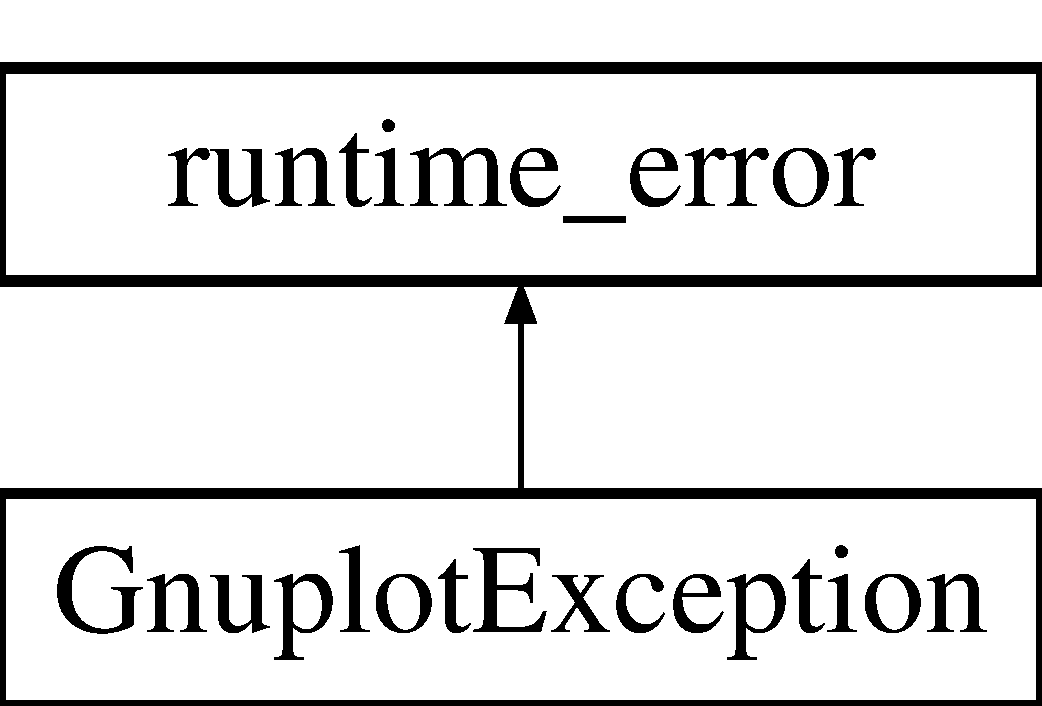
\includegraphics[height=2.000000cm]{d1/dd4/class_gnuplot_exception}
\end{center}
\end{figure}
\subsection*{Public Member Functions}
\begin{DoxyCompactItemize}
\item 
\textbf{ Gnuplot\+Exception} (const std\+::string \&msg)
\end{DoxyCompactItemize}


\subsection{Detailed Description}
A C++ interface to gnuplot. 

The interface uses pipes and so won\textquotesingle{}t run on a system that doesn\textquotesingle{}t have P\+O\+S\+IX pipe support Tested on Windows (Min\+GW and Visual C++) and Linux (G\+CC)

Version history\+: 0. C interface by N. Devillard (27/01/03)
\begin{DoxyEnumerate}
\item C++ interface\+: direct translation from the C interface by Rajarshi Guha (07/03/03)
\item corrections for Win32 compatibility by V. Chyzhdzenka (20/05/03)
\item some member functions added, corrections for Win32 and Linux compatibility by M. Burgis (10/03/08)
\end{DoxyEnumerate}

Requirements\+:
\begin{DoxyItemize}
\item gnuplot has to be installed ({\tt http\+://www.\+gnuplot.\+info/download.\+html})
\item for Windows\+: set Path-\/\+Variable for \doxyref{Gnuplot}{p.}{d3/d27/class_gnuplot} path (e.\+g. C\+:/program files/gnuplot/bin) or set \doxyref{Gnuplot}{p.}{d3/d27/class_gnuplot} path with\+: \doxyref{Gnuplot\+::set\+\_\+\+G\+N\+U\+Plot\+Path(const std\+::string \&path)}{p.}{d3/d27/class_gnuplot_a67cae885c26ced821e335d98986f1967}; 
\end{DoxyItemize}

Definition at line 60 of file gnuplot\+\_\+i.\+hpp.



\subsection{Constructor \& Destructor Documentation}
\mbox{\label{class_gnuplot_exception_a8b324a9ef4d3f75079d41ecd61c62d44}} 
\index{Gnuplot\+Exception@{Gnuplot\+Exception}!Gnuplot\+Exception@{Gnuplot\+Exception}}
\index{Gnuplot\+Exception@{Gnuplot\+Exception}!Gnuplot\+Exception@{Gnuplot\+Exception}}
\subsubsection{Gnuplot\+Exception()}
{\footnotesize\ttfamily Gnuplot\+Exception\+::\+Gnuplot\+Exception (\begin{DoxyParamCaption}\item[{const std\+::string \&}]{msg }\end{DoxyParamCaption})\hspace{0.3cm}{\ttfamily [inline]}}



Definition at line 63 of file gnuplot\+\_\+i.\+hpp.


\begin{DoxyCode}
63 : std::runtime\_error(msg)\{\}
\end{DoxyCode}


The documentation for this class was generated from the following file\+:\begin{DoxyCompactItemize}
\item 
\textbf{ gnuplot\+\_\+i.\+hpp}\end{DoxyCompactItemize}

\chapter{File Documentation}
\section{example.\+cc File Reference}
\label{example_8cc}\index{example.\+cc@{example.\+cc}}
{\ttfamily \#include $<$iostream$>$}\newline
{\ttfamily \#include \char`\"{}gnuplot\+\_\+i.\+hpp\char`\"{}}\newline
\subsection*{Macros}
\begin{DoxyCompactItemize}
\item 
\#define \textbf{ S\+L\+E\+E\+P\+\_\+\+L\+G\+TH}~2
\item 
\#define \textbf{ N\+P\+O\+I\+N\+TS}~50
\end{DoxyCompactItemize}
\subsection*{Functions}
\begin{DoxyCompactItemize}
\item 
void \textbf{ wait\+\_\+for\+\_\+key} ()
\item 
int \textbf{ main} (int argc, char $\ast$argv[$\,$])
\end{DoxyCompactItemize}


\subsection{Macro Definition Documentation}
\mbox{\label{example_8cc_a046c61fd31a06b2051fa0f57e626ee65}} 
\index{example.\+cc@{example.\+cc}!N\+P\+O\+I\+N\+TS@{N\+P\+O\+I\+N\+TS}}
\index{N\+P\+O\+I\+N\+TS@{N\+P\+O\+I\+N\+TS}!example.\+cc@{example.\+cc}}
\subsubsection{N\+P\+O\+I\+N\+TS}
{\footnotesize\ttfamily \#define N\+P\+O\+I\+N\+TS~50}



Definition at line 20 of file example.\+cc.



Referenced by main().

\mbox{\label{example_8cc_a86c9f48acee3e4ad980ffbaacc293a1a}} 
\index{example.\+cc@{example.\+cc}!S\+L\+E\+E\+P\+\_\+\+L\+G\+TH@{S\+L\+E\+E\+P\+\_\+\+L\+G\+TH}}
\index{S\+L\+E\+E\+P\+\_\+\+L\+G\+TH@{S\+L\+E\+E\+P\+\_\+\+L\+G\+TH}!example.\+cc@{example.\+cc}}
\subsubsection{S\+L\+E\+E\+P\+\_\+\+L\+G\+TH}
{\footnotesize\ttfamily \#define S\+L\+E\+E\+P\+\_\+\+L\+G\+TH~2}



Definition at line 19 of file example.\+cc.



\subsection{Function Documentation}
\mbox{\label{example_8cc_a0ddf1224851353fc92bfbff6f499fa97}} 
\index{example.\+cc@{example.\+cc}!main@{main}}
\index{main@{main}!example.\+cc@{example.\+cc}}
\subsubsection{main()}
{\footnotesize\ttfamily int main (\begin{DoxyParamCaption}\item[{int}]{argc,  }\item[{char $\ast$}]{argv[$\,$] }\end{DoxyParamCaption})}



Definition at line 27 of file example.\+cc.



References Gnuplot\+::cmd(), N\+P\+O\+I\+N\+TS, Gnuplot\+::plot\+\_\+equation(), Gnuplot\+::plot\+\_\+equation3d(), Gnuplot\+::plot\+\_\+image(), Gnuplot\+::plot\+\_\+slope(), Gnuplot\+::plot\+\_\+x(), Gnuplot\+::plot\+\_\+xy(), Gnuplot\+::plot\+\_\+xy\+\_\+err(), Gnuplot\+::plot\+\_\+xyz(), Gnuplot\+::replot(), Gnuplot\+::reset\+\_\+all(), Gnuplot\+::reset\+\_\+plot(), Gnuplot\+::savetops(), Gnuplot\+::set\+\_\+cbrange(), Gnuplot\+::set\+\_\+contour(), Gnuplot\+::set\+\_\+grid(), Gnuplot\+::set\+\_\+hidden3d(), Gnuplot\+::set\+\_\+isosamples(), Gnuplot\+::set\+\_\+legend(), Gnuplot\+::set\+\_\+pointsize(), Gnuplot\+::set\+\_\+samples(), Gnuplot\+::set\+\_\+smooth(), Gnuplot\+::set\+\_\+style(), Gnuplot\+::set\+\_\+surface(), Gnuplot\+::set\+\_\+title(), Gnuplot\+::set\+\_\+xautoscale(), Gnuplot\+::set\+\_\+xlabel(), Gnuplot\+::set\+\_\+xrange(), Gnuplot\+::set\+\_\+ylabel(), Gnuplot\+::set\+\_\+yrange(), Gnuplot\+::set\+\_\+zlabel(), Gnuplot\+::set\+\_\+zrange(), Gnuplot\+::showonscreen(), Gnuplot\+::unset\+\_\+grid(), Gnuplot\+::unset\+\_\+legend(), Gnuplot\+::unset\+\_\+smooth(), Gnuplot\+::unset\+\_\+surface(), Gnuplot\+::unset\+\_\+title(), and wait\+\_\+for\+\_\+key().


\begin{DoxyCode}
28 \{
29     \textcolor{comment}{// if path-variable for gnuplot is not set, do it with:}
30     \textcolor{comment}{// Gnuplot::set\_GNUPlotPath("C:/program files/gnuplot/bin/");}
31 
32     \textcolor{comment}{// set a special standard terminal for showonscreen (normally not needed),}
33     \textcolor{comment}{//   e.g. Mac users who want to use x11 instead of aqua terminal:}
34     \textcolor{comment}{// Gnuplot::set\_terminal\_std("x11");}
35 
36     cout << \textcolor{stringliteral}{"*** example of gnuplot control through C++ ***"} << endl << endl;
37 
38     \textcolor{comment}{//}
39     \textcolor{comment}{// Using the GnuplotException class}
40     \textcolor{comment}{//}
41     \textcolor{keywordflow}{try}
42     \{
43         Gnuplot g1(\textcolor{stringliteral}{"lines"});
44 
45         \textcolor{comment}{//}
46         \textcolor{comment}{// Slopes}
47         \textcolor{comment}{//}
48         cout << \textcolor{stringliteral}{"*** plotting slopes"} << endl;
49         g1.set\_title(\textcolor{stringliteral}{"Slopes\(\backslash\)\(\backslash\)nNew Line"});
50 
51         cout << \textcolor{stringliteral}{"y = x"} << endl;
52         g1.plot\_slope(1.0,0.0,\textcolor{stringliteral}{"y=x"});
53 
54         cout << \textcolor{stringliteral}{"y = 2*x"} << endl;
55         g1.plot\_slope(2.0,0.0,\textcolor{stringliteral}{"y=2x"});
56 
57         cout << \textcolor{stringliteral}{"y = -x"} << endl;
58         g1.plot\_slope(-1.0,0.0,\textcolor{stringliteral}{"y=-x"});
59         g1.unset\_title();
60 
61         \textcolor{comment}{//}
62         \textcolor{comment}{// Equations}
63         \textcolor{comment}{//}
64         g1.reset\_plot();
65         cout << endl << endl << \textcolor{stringliteral}{"*** various equations"} << endl;
66 
67         cout << \textcolor{stringliteral}{"y = sin(x)"} << endl;
68         g1.plot\_equation(\textcolor{stringliteral}{"sin(x)"},\textcolor{stringliteral}{"sine"});
69 
70         cout << \textcolor{stringliteral}{"y = log(x)"} << endl;
71         g1.plot\_equation(\textcolor{stringliteral}{"log(x)"},\textcolor{stringliteral}{"logarithm"});
72 
73         cout << \textcolor{stringliteral}{"y = sin(x) * cos(2*x)"} << endl;
74         g1.plot\_equation(\textcolor{stringliteral}{"sin(x)*cos(2*x)"},\textcolor{stringliteral}{"sine product"});
75 
76         \textcolor{comment}{//}
77         \textcolor{comment}{// Styles}
78         \textcolor{comment}{//}
79         g1.reset\_plot();
80         cout << endl << endl << \textcolor{stringliteral}{"*** showing styles"} << endl;
81 
82         cout << \textcolor{stringliteral}{"sine in points"} << endl;
83         g1.set\_pointsize(0.8).set\_style(\textcolor{stringliteral}{"points"});
84         g1.plot\_equation(\textcolor{stringliteral}{"sin(x)"},\textcolor{stringliteral}{"points"});
85 
86         cout << \textcolor{stringliteral}{"sine in impulses"} << endl;
87         g1.set\_style(\textcolor{stringliteral}{"impulses"});
88         g1.plot\_equation(\textcolor{stringliteral}{"sin(x)"},\textcolor{stringliteral}{"impulses"});
89 
90         cout << \textcolor{stringliteral}{"sine in steps"} << endl;
91         g1.set\_style(\textcolor{stringliteral}{"steps"});
92         g1.plot\_equation(\textcolor{stringliteral}{"sin(x)"},\textcolor{stringliteral}{"steps"});
93 
94         \textcolor{comment}{//}
95         \textcolor{comment}{// Save to ps}
96         \textcolor{comment}{//}
97         g1.reset\_all();
98         cout << endl << endl << \textcolor{stringliteral}{"*** save to ps "} << endl;
99 
100         cout << \textcolor{stringliteral}{"y = sin(x) saved to test\_output.ps in working directory"} << endl;
101         g1.savetops(\textcolor{stringliteral}{"test\_output"});
102         g1.set\_style(\textcolor{stringliteral}{"lines"}).set\_samples(300).set\_xrange(0,5);
103         g1.plot\_equation(\textcolor{stringliteral}{"sin(12*x)*exp(-x)"}).plot\_equation(\textcolor{stringliteral}{"exp(-x)"});
104 
105         g1.showonscreen(); \textcolor{comment}{// window output}
106 
107 
108         \textcolor{comment}{//}
109         \textcolor{comment}{// User defined 1d, 2d and 3d point sets}
110         \textcolor{comment}{//}
111         std::vector<double> x, y, y2, dy, z;
112 
113         \textcolor{keywordflow}{for} (\textcolor{keywordtype}{int} i = 0; i < NPOINTS; i++)  \textcolor{comment}{// fill double arrays x, y, z}
114         \{
115             x.push\_back((\textcolor{keywordtype}{double})i);             \textcolor{comment}{// x[i] = i}
116             y.push\_back((\textcolor{keywordtype}{double})i * (\textcolor{keywordtype}{double})i); \textcolor{comment}{// y[i] = i^2}
117             z.push\_back( x[i]*y[i] );           \textcolor{comment}{// z[i] = x[i]*y[i] = i^3}
118             dy.push\_back((\textcolor{keywordtype}{double})i * (\textcolor{keywordtype}{double})i / (\textcolor{keywordtype}{double}) 10); \textcolor{comment}{// dy[i] = i^2 / 10}
119         \}
120         y2.push\_back(0.00); y2.push\_back(0.78); y2.push\_back(0.97); y2.push\_back(0.43);
121         y2.push\_back(-0.44); y2.push\_back(-0.98); y2.push\_back(-0.77); y2.push\_back(0.02);
122 
123 
124         g1.reset\_all();
125         cout << endl << endl << \textcolor{stringliteral}{"*** user-defined lists of doubles"} << endl;
126         g1.set\_style(\textcolor{stringliteral}{"impulses"}).plot\_x(y,\textcolor{stringliteral}{"user-defined doubles"});
127 
128         g1.reset\_plot();
129         cout << endl << endl << \textcolor{stringliteral}{"*** user-defined lists of points (x,y)"} << endl;
130         g1.set\_grid();
131         g1.set\_style(\textcolor{stringliteral}{"points"}).plot\_xy(x,y,\textcolor{stringliteral}{"user-defined points 2d"});
132 
133         g1.reset\_plot();
134         cout << endl << endl << \textcolor{stringliteral}{"*** user-defined lists of points (x,y,z)"} << endl;
135         g1.unset\_grid();
136         g1.plot\_xyz(x,y,z,\textcolor{stringliteral}{"user-defined points 3d"});
137 
138         g1.reset\_plot();
139         cout << endl << endl << \textcolor{stringliteral}{"*** user-defined lists of points (x,y,dy)"} << endl;
140         g1.plot\_xy\_err(x,y,dy,\textcolor{stringliteral}{"user-defined points 2d with errorbars"});
141 
142 
143         \textcolor{comment}{//}
144         \textcolor{comment}{// Multiple output screens}
145         \textcolor{comment}{//}
146         cout << endl << endl;
147         cout << \textcolor{stringliteral}{"*** multiple output windows"} << endl;
148 
149         g1.reset\_plot();
150         g1.set\_style(\textcolor{stringliteral}{"lines"});
151         cout << \textcolor{stringliteral}{"window 1: sin(x)"} << endl;
152         g1.set\_grid().set\_samples(600).set\_xrange(0,300);
153         g1.plot\_equation(\textcolor{stringliteral}{"sin(x)+sin(x*1.1)"});
154 
155         g1.set\_xautoscale().replot();
156 
157         Gnuplot g2;
158         cout << \textcolor{stringliteral}{"window 2: user defined points"} << endl;
159         g2.plot_x(y2,\textcolor{stringliteral}{"points"});
160         g2.set_smooth().plot_x(y2,\textcolor{stringliteral}{"cspline"});
161         g2.set_smooth(\textcolor{stringliteral}{"bezier"}).plot_x(y2,\textcolor{stringliteral}{"bezier"});
162         g2.unset_smooth();
163 
164         Gnuplot g3(\textcolor{stringliteral}{"lines"});
165         cout << \textcolor{stringliteral}{"window 3: log(x)/x"} << endl;
166         g3.set\_grid();
167         g3.plot\_equation(\textcolor{stringliteral}{"log(x)/x"},\textcolor{stringliteral}{"log(x)/x"});
168 
169         Gnuplot g4(\textcolor{stringliteral}{"lines"});
170         cout << \textcolor{stringliteral}{"window 4: splot x*x+y*y"} << endl;
171         g4.set\_zrange(0,100);
172         g4.set\_xlabel(\textcolor{stringliteral}{"x-axis"}).set\_ylabel(\textcolor{stringliteral}{"y-axis"}).set\_zlabel(\textcolor{stringliteral}{"z-axis"});
173         g4.plot\_equation3d(\textcolor{stringliteral}{"x*x+y*y"});
174 
175         Gnuplot g5(\textcolor{stringliteral}{"lines"});
176         cout << \textcolor{stringliteral}{"window 5: splot with hidden3d"} << endl;
177         g5.set\_isosamples(25).set\_hidden3d();
178         g5.plot\_equation3d(\textcolor{stringliteral}{"x*y*y"});
179 
180         Gnuplot g6(\textcolor{stringliteral}{"lines"});
181         cout << \textcolor{stringliteral}{"window 6: splot with contour"} << endl;
182         g6.set\_isosamples(60).set\_contour();
183         g6.unset\_surface().plot\_equation3d(\textcolor{stringliteral}{"sin(x)*sin(y)+4"});
184 
185         g6.set\_surface().replot();
186 
187         Gnuplot g7(\textcolor{stringliteral}{"lines"});
188         cout << \textcolor{stringliteral}{"window 7: set\_samples"} << endl;
189         g7.set\_xrange(-30,20).set\_samples(40);
190         g7.plot\_equation(\textcolor{stringliteral}{"besj0(x)*0.12e1"}).plot\_equation(\textcolor{stringliteral}{"(x**besj0(x))-2.5"});
191 
192         g7.set\_samples(400).replot();
193 
194         Gnuplot g8(\textcolor{stringliteral}{"filledcurves"});
195         cout << \textcolor{stringliteral}{"window 8: filledcurves"} << endl;
196         g8.set\_legend(\textcolor{stringliteral}{"outside right top"}).set\_xrange(-5,5);
197         g8.plot\_equation(\textcolor{stringliteral}{"x*x"}).plot\_equation(\textcolor{stringliteral}{"-x*x+4"});
198 
199         \textcolor{comment}{//}
200         \textcolor{comment}{// Plot an image}
201         \textcolor{comment}{//}
202         Gnuplot g9;
203         cout << \textcolor{stringliteral}{"window 9: plot\_image"} << endl;
204         \textcolor{keyword}{const} \textcolor{keywordtype}{int} iWidth  = 255;
205         \textcolor{keyword}{const} \textcolor{keywordtype}{int} iHeight = 255;
206         g9.set_xrange(0,iWidth).set_yrange(0,iHeight).set_cbrange(0,255);
207         g9.cmd(\textcolor{stringliteral}{"set palette gray"});
208         \textcolor{keywordtype}{unsigned} \textcolor{keywordtype}{char} ucPicBuf[iWidth*iHeight];
209         \textcolor{comment}{// generate a greyscale image}
210         \textcolor{keywordflow}{for}(\textcolor{keywordtype}{int} iIndex = 0; iIndex < iHeight*iWidth; iIndex++)
211         \{
212             ucPicBuf[iIndex] = iIndex%255;
213         \}
214         g9.plot_image(ucPicBuf,iWidth,iHeight,\textcolor{stringliteral}{"greyscale"});
215 
216         g9.set_pointsize(0.6).unset_legend().plot_slope(0.8,20);
217 
218         \textcolor{comment}{//}
219         \textcolor{comment}{// manual control}
220         \textcolor{comment}{//}
221         Gnuplot g10;
222         cout << \textcolor{stringliteral}{"window 10: manual control"} << endl;
223         g10.cmd(\textcolor{stringliteral}{"set samples 400"}).cmd(\textcolor{stringliteral}{"plot abs(x)/2"}); \textcolor{comment}{// either with cmd()}
224         g10 << \textcolor{stringliteral}{"replot sqrt(x)"} << \textcolor{stringliteral}{"replot sqrt(-x)"};    \textcolor{comment}{// or with <<}
225 
226         wait_for_key();
227 
228     \}
229     \textcolor{keywordflow}{catch} (GnuplotException ge)
230     \{
231         cout << ge.what() << endl;
232     \}
233 
234 
235     cout << endl << \textcolor{stringliteral}{"*** end of gnuplot example"} << endl;
236 
237     \textcolor{keywordflow}{return} 0;
238 \}
\end{DoxyCode}
\mbox{\label{example_8cc_a621288a08ecc9633729935737256e831}} 
\index{example.\+cc@{example.\+cc}!wait\+\_\+for\+\_\+key@{wait\+\_\+for\+\_\+key}}
\index{wait\+\_\+for\+\_\+key@{wait\+\_\+for\+\_\+key}!example.\+cc@{example.\+cc}}
\subsubsection{wait\+\_\+for\+\_\+key()}
{\footnotesize\ttfamily void wait\+\_\+for\+\_\+key (\begin{DoxyParamCaption}{ }\end{DoxyParamCaption})}



Definition at line 242 of file example.\+cc.



Referenced by main().


\begin{DoxyCode}
243 \{
244 \textcolor{preprocessor}{#if defined(WIN32) || defined(\_WIN32) || defined(\_\_WIN32\_\_) || defined(\_\_TOS\_WIN\_\_)  // every keypress
       registered, also arrow keys}
245     cout << endl << \textcolor{stringliteral}{"Press any key to continue..."} << endl;
246 
247     FlushConsoleInputBuffer(GetStdHandle(STD\_INPUT\_HANDLE));
248     \_getch();
249 \textcolor{preprocessor}{#elif defined(unix) || defined(\_\_unix) || defined(\_\_unix\_\_) || defined(\_\_APPLE\_\_)}
250     cout << endl << \textcolor{stringliteral}{"Press ENTER to continue..."} << endl;
251 
252     std::cin.clear();
253     std::cin.ignore(std::cin.rdbuf()->in\_avail());
254     std::cin.get();
255 \textcolor{preprocessor}{#endif}
256     \textcolor{keywordflow}{return};
257 \}
\end{DoxyCode}

\section{gnuplot\+\_\+i.\+hpp File Reference}
\label{gnuplot__i_8hpp}\index{gnuplot\+\_\+i.\+hpp@{gnuplot\+\_\+i.\+hpp}}
{\ttfamily \#include $<$iostream$>$}\newline
{\ttfamily \#include $<$string$>$}\newline
{\ttfamily \#include $<$vector$>$}\newline
{\ttfamily \#include $<$fstream$>$}\newline
{\ttfamily \#include $<$sstream$>$}\newline
{\ttfamily \#include $<$stdexcept$>$}\newline
{\ttfamily \#include $<$cstdio$>$}\newline
{\ttfamily \#include $<$cstdlib$>$}\newline
{\ttfamily \#include $<$list$>$}\newline
\subsection*{Classes}
\begin{DoxyCompactItemize}
\item 
class \textbf{ Gnuplot\+Exception}
\begin{DoxyCompactList}\small\item\em A C++ interface to gnuplot. \end{DoxyCompactList}\item 
class \textbf{ Gnuplot}
\end{DoxyCompactItemize}
\subsection*{Functions}
\begin{DoxyCompactItemize}
\item 
{\footnotesize template$<$typename Container $>$ }\\void \textbf{ stringtok} (Container \&container, std\+::string const \&in, const char $\ast$const delimiters=\char`\"{} \textbackslash{}\char`\"{})
\end{DoxyCompactItemize}


\subsection{Function Documentation}
\mbox{\label{gnuplot__i_8hpp_aa638112596d8394216cd0954f18fb676}} 
\index{gnuplot\+\_\+i.\+hpp@{gnuplot\+\_\+i.\+hpp}!stringtok@{stringtok}}
\index{stringtok@{stringtok}!gnuplot\+\_\+i.\+hpp@{gnuplot\+\_\+i.\+hpp}}
\subsubsection{stringtok()}
{\footnotesize\ttfamily template$<$typename Container $>$ \\
void stringtok (\begin{DoxyParamCaption}\item[{Container \&}]{container,  }\item[{std\+::string const \&}]{in,  }\item[{const char $\ast$const}]{delimiters = {\ttfamily \char`\"{}~\textbackslash{}t\textbackslash{}n\char`\"{}} }\end{DoxyParamCaption})}



Definition at line 905 of file gnuplot\+\_\+i.\+hpp.



Referenced by Gnuplot\+::cmd().


\begin{DoxyCode}
908 \{
909     \textcolor{keyword}{const} std::string::size\_type len = in.length();
910           std::string::size\_type i = 0;
911 
912     \textcolor{keywordflow}{while} ( i < len )
913     \{
914         \textcolor{comment}{// eat leading whitespace}
915         i = in.find\_first\_not\_of (delimiters, i);
916 
917         \textcolor{keywordflow}{if} (i == std::string::npos)
918             \textcolor{keywordflow}{return};   \textcolor{comment}{// nothing left but white space}
919 
920         \textcolor{comment}{// find the end of the token}
921         std::string::size\_type j = in.find\_first\_of (delimiters, i);
922 
923         \textcolor{comment}{// push token}
924         \textcolor{keywordflow}{if} (j == std::string::npos)
925         \{
926             container.push\_back (in.substr(i));
927             \textcolor{keywordflow}{return};
928         \}
929         \textcolor{keywordflow}{else}
930             container.push\_back (in.substr(i, j-i));
931 
932         \textcolor{comment}{// set up for next loop}
933         i = j + 1;
934     \}
935 
936     \textcolor{keywordflow}{return};
937 \}
\end{DoxyCode}

%--- End generated contents ---

% Index
\backmatter
\newpage
\phantomsection
\clearemptydoublepage
\addcontentsline{toc}{chapter}{Index}
\printindex

\end{document}
